%%% Exemplo de utilização da classe ITA
%%%
%%%   por        Fábio Fagundes Silveira   -  ffs [at] ita [dot] br
%%%              Benedito C. O. Maciel     -  bcmaciel [at] ita [dot] br
%%%              Giovani Volnei Meinertz   -  giovani [at] ita [dot] br
%%%    	         Hudson Alberto Bode       -  bode [at] ita [dot]br
%%%    	         P. I. Braga de Queiroz    -  pi [at] ita [dot] br
%%%    	         Jorge A. B. Gripp         -  gripp [at] ita [dot] br
%%%    	         Juliano Monte-Mor         -  jamontemor [at] yahoo [dot] com [dot] br
%%%    	         Tarcisio A. B. Gripp      -  tarcisio.gripp [at] gmail [dot] com
%%%
%%%   Versão para overleaf:
%%%   por        Alejandro A. Rios Cruz    - aarc.88@gmail.com
%%%              Saulo Gómez               - sagomezs@unal.edu.co
%%%              Ocimar Santos             - ocimar.acad@gmail.com
%%%
%%%   Template disponibilizado em:
%%%              Overleaf: https://pt.overleaf.com/latex/templates/thesis-template-aeronautics-institute-of-technology-ita/yhfrqqydpygk
%%%
%%%   Contribuia você também!
%%%              GitHub:   https://github.com/AlejandroRios/Template_Thesis_ITA
%%%
%%% ITALUS
%%% Instituto Tecnológico de Aeronáutica --- ITA, Sao Jose dos Campos, Brasil
%%%
%++++++++++++++++++++++++++++++++++++++++++++++++++++++++++++++++++++++++++++++
% Para alterar o TIPO DE DOCUMENTO, preencher a linha abaixo \documentclass[?]{?}
%   \documentclass[tg]{ita}			= Trabalho de Graduacao
%   \documentclass[tgfem]{ita}	= Para Engenheiras
%   								msc     		= Dissertacao de Mestrado
%   								mscfem   		= Para Mestras
%   								dsc      		= Tese de Doutorado
%   								dscfem   		= Para Doutoras
%   								quali    		= Exame de Qualificacao
%   								qualifem 		= Exame de Qualificacao para Doutoras
% Para 'Draft Version'/'Versao Preliminar' com data no rodape, adicionar 'dv':
%   \documentclass[dsc, dv]{ita}
% Para trabalhos em Inglês, adicionar 'eng':
%   \documentclass[dsc, eng]{ita}
%++++++++++++++++++++++++++++++++++++++++++++++++++++++++++++++++++++++++++++++
\documentclass[msc, eng]{ita}    % Dissertação de Mestrado, em inglês
% Ao alterar a classe, rode o BUILD mais uma vez caso apareça algum erro.
\usepackage{ae}
\usepackage{graphicx}
\usepackage{epsfig}
\usepackage{amsmath}
\usepackage{amssymb}
\usepackage{subfig}
\usepackage{multirow}
\usepackage{float}
\usepackage{amsthm}
\usepackage{url}         % formats URL addresses properly
\usepackage{appendix}    % allows appendix section to be included
\usepackage{lscape}      % allows a page to be rendered in landscape mode
\usepackage{multicol}    % allows text in multi columns
\usepackage{cancel}      % needed to show canceled terms in equations
\usepackage{lettrine}
\usepackage{float}
\usepackage{placeins}

\usepackage{caption}
% \usepackage{subcaption} % conflicts with subfig (both loaded, neither used); subfig is kept

\usepackage{booktabs}
\usepackage{bm}          % bold math symbols for vectors/matrices

% Theorem-like environments (used in the methodology chapters)
\newtheorem{proposition}{Proposition}[chapter]
\newtheorem{lemma}{Lemma}[chapter]
\theoremstyle{remark}
\newtheorem{remark}{Remark}[chapter]

%++++++++++++++++++++++++++++++++++++++++++++++++++++++++++++++++++++++++++++++
% Espaçamento padrão de todo o documento
%++++++++++++++++++++++++++++++++++++++++++++++++++++++++++++++++++++++++++++++
\onehalfspacing

%++++++++++++++++++++++++++++++++++++++++++++++++++++++++++++++++++++++++++++++
% Quebra de linha: evita palavras ultrapassando a margem direita.
% Compostos já hifenizados ("three-dimensional", "camera--LiDAR") não podem ser
% hifenizados novamente pelo TeX, o que produzia linhas "overfull". O
% \emergencystretch permite que o TeX estique o espaçamento entre palavras num
% último passe, em vez de estourar a margem.
%++++++++++++++++++++++++++++++++++++++++++++++++++++++++++++++++++++++++++++++
\tolerance=2000
\emergencystretch=3em

%++++++++++++++++++++++++++++++++++++++++++++++++++++++++++++++++++++++++++++++
% Identificações (trabalho em inglês -> dados em inglês)
%++++++++++++++++++++++++++++++++++++++++++++++++++++++++++++++++++++++++++++++
\course{Electronic Engineering and Computer Science}  % Programa de PG em Engenharia Eletrônica e Computação
\area{Informatics}                                    % Área de Informática

% Autor do trabalho: Nome Sobrenome
\authorgender{masc}                     % masc ou fem
\author{Eric Ezequiel Yoshida}{de Lima}
\itaauthoraddress{Rua H8B, Ap. 216}{12.228-461}{São José dos Campos--SP}

% Título da Dissertação (atualizado conforme revisão do orientador)
\title{Object Detection and Tracking Using an Unmanned Aerial Vehicle}

% Orientador
\advisorgender{masc}                    % masc ou fem
\advisor{Prof.~Dr.}{Marcos Ricardo Omena de Albuquerque Maximo}{ITA}

% Coorientador
\coadvisorgender{masc}                  % masc ou fem
\coadvisor{Dr.}{Stiven Schwanz Dias}{Embraer S.A.}

% Pró-reitor da Pós-graduação
\bossgender{masc}                       % masc ou fem
\boss{Prof.~Dr.}{André Valdetaro Gomes Cavalieri}   % Pró-Reitor de Pós-Graduação do ITA

% Coordenador do curso -> somente TG (não se aplica a mestrado)
%\bosscoursegender{masc}
%\bosscourse{Prof.~Dr.}{}

% Palavras-Chaves informadas pela Biblioteca -> utilizada na CIP
\kwcip{Unmanned aerial vehicles}
\kwcip{Detect-and-avoid}
\kwcip{Object tracking}
\kwcip{Extended Kalman filter}
\kwcip{3D object detection}
\kwcip{Sensor fusion}
\kwcip{Convolutional neural networks}

% Membros da banca examinadora (a ordem na folha: Presidente, Orientador, Coorientador, demais membros)
\examiner{Prof.~Dr.}{Paulo Marcelo Tasinaffo}{President}{ITA}
\examiner{Prof.~Dr.}{Marcelo Gomes da Silva Bruno}{Internal Member}{ITA}
\examiner{Prof.~Dr.}{Alberto Ferreira de Souza}{External Member}{UFES}
\examiner{Prof.~Dr.}{Cesar Augusto Cavalheiro Marcondes}{Internal Substitute}{ITA}
\examiner{Prof.~Dr.}{Thiago Oliveira Santos}{External Substitute}{UFES}

% Data da defesa (mês em maiúsculo, pois o trabalho é em inglês)
\date{28}{July}{2026}                   % Data da defesa

% Número CDU -> somente TG (não se aplica a mestrado)
%\cdu{}

% Glossário
\makeglossary
\frontmatter

\begin{document}
% Folha de Rosto e Capa para o caso do TG
\maketitle

% Dedicatoria: Nao esqueca essa secao  ... :-)
\begin{itadedication}
To my friends from the undergraduate and graduate programs at ITA and to my
professors who supported me in this work, and to my family, who has always
supported me throughout this long journey.
\end{itadedication}

% Agradecimentos
\begin{itathanks}
% Agradecimentos.

I am deeply grateful to my advisor, Prof.\ Dr.\ Marcos R.\ O.\ A.\ M\'aximo, and
my co-advisor, Prof.\ Dr.\ Stiven S.\ Dias, for their guidance, patience, and
careful reading of this work. Their insight shaped both the research and the way
it is presented here.

This work was carried out within the FlyMov Engineering Research Center, a
partnership between the Aeronautics Institute of Technology (ITA), Embraer, and
the S\~ao Paulo Research Foundation (FAPESP), whose support made the research
possible.

I thank the UBADRON team of the Chair of Flight Guidance and Air Transport at the
Technische Universit\"at Berlin (TU~Berlin), led by Prof.\ Dr.\ Maarten Uijt de
Haag, for hosting me during my research stay and for the collaboration that made
the real-world study of Chapter~\ref{cha:monocular} possible. I am especially
grateful to Anne-Sophie Polz for sharing the flight data and for her help with
the experiments.

Finally, I thank my family and friends for their constant encouragement and
support throughout this journey.

\end{itathanks}

% Epígrafe
\thispagestyle{empty}
\ifhyperref\pdfbookmark[0]{\nameepigraphe}{epigrafe}\fi
\begin{flushright}
\begin{spacing}{1}
\mbox{}\vfill
{\sffamily\itshape
``Artificial intelligence is the new electricity.''\\}
--- \textsc{ANDREW NG}

\end{spacing}
\end{flushright}

% Resumo
\begin{abstract}
\noindent
% Resumo (português) --- obrigatório pelo ITA mesmo em dissertações escritas em inglês.
% TODO: escrever o resumo (~150--250 palavras) ao final, espelhando o Abstract.
[Resumo a preencher: contexto (sense-and-avoid / consciência situacional para eVTOLs urbanos), problema (detecção e rastreamento 3D a partir de plataforma aérea em movimento), abordagem (pipeline modular câmera--nuvem de pontos; tracker baseado em EKF validado em simulação e em dados reais), e principais resultados.]

\end{abstract}

% Abstract
\begin{englishabstract}
\noindent
% Abstract (English).
% TODO: write the abstract (~150--250 words) once results are consolidated.
[Abstract to be written: context (sense-and-avoid / situational awareness for urban eVTOLs), problem (3D obstacle detection and tracking from a moving aerial platform), approach (a modular camera--point-cloud perception pipeline; an EKF-based tracker validated in simulation and on real data), and main results.]

\end{englishabstract}

% Lista de figuras
\listoffigures %opcional

% Lista de tabelas
\listoftables %opcional

% Lista de abreviaturas
\listofabbreviations
% Lista de abreviaturas (mantida manualmente).
\begin{longtable}{ll}
AI      & Artificial Intelligence \\
AirSim  & Aerial Informatics and Robotics Simulation \\
AMOTA   & Average Multi-Object-Tracking Accuracy \\
AMOTP   & Average Multi-Object-Tracking Precision \\
BEV     & Bird's-Eye View \\
CNN     & Convolutional Neural Network \\
CRLB    & Cram\'er--Rao Lower Bound \\
CV      & Constant-Velocity (motion model) \\
D\&A    & Detect-and-Avoid \\
EKF     & Extended Kalman Filter \\
ENU     & East--North--Up (reference frame) \\
eVTOL   & Electric Vertical Take-Off and Landing \\
FIM     & Fisher Information Matrix \\
FN      & False Negative \\
FP      & False Positive \\
GNSS    & Global Navigation Satellite System \\
HSV     & Hue--Saturation--Value (color space) \\
IDF1    & Identity F1 Score \\
IMU     & Inertial Measurement Unit \\
IoU     & Intersection over Union \\
KF      & Kalman Filter \\
LiDAR   & Light Detection and Ranging \\
mAP     & Mean Average Precision \\
MLP     & Multilayer Perceptron \\
MOT     & Multi-Object Tracking \\
MOTA    & Multi-Object-Tracking Accuracy \\
NED     & North--East--Down (reference frame) \\
NEES    & Normalized Estimation Error Squared \\
NIS     & Normalized Innovation Squared \\
NMS     & Non-Maximum Suppression \\
PCRB    & Posterior Cram\'er--Rao Bound \\
PFN     & Pillar Feature Network \\
PICOC   & Population, Intervention, Comparison, Outcome, Context \\
PRISMA  & Preferred Reporting Items for Systematic Reviews and Meta-Analyses \\
RGB     & Red--Green--Blue (image) \\
RGB-D   & Red--Green--Blue--Depth (image) \\
RMSE    & Root-Mean-Square Error \\
RPC     & Remote-Procedure Call \\
SA      & Set-Abstraction (PointNet\texttt{++} level) \\
SGD     & Stochastic Gradient Descent \\
SLERP   & Spherical Linear Interpolation \\
SLR     & Systematic Literature Review \\
SORT    & Simple Online and Realtime Tracking \\
TP      & True Positive \\
UAM     & Urban Air Mobility \\
UAV     & Unmanned Aerial Vehicle \\
UKF     & Unscented Kalman Filter \\
YOLO    & You Only Look Once \\
\end{longtable}
 %opcional

% Lista de simbolos
\listofsymbols
% Lista de símbolos (mantida manualmente). Conjunto inicial; completar conforme o texto.
\begin{longtable}{ll}
$\bm{x}_k$        & State vector at time $k$ \\
$\bm{F}$          & State-transition matrix \\
$\bm{G}$          & Process-noise gain matrix \\
$\bm{Q}$          & Process-noise covariance matrix \\
$\bm{H}_k$        & Measurement Jacobian \\
$\bm{P}_{k|k}$    & State (posterior) covariance matrix \\
$\bm{R}_k$        & Measurement-noise covariance matrix \\
$\bm{K}_k$        & Kalman gain \\
$\bm{z}_k$        & Measurement vector \\
$\bm{\nu}_k$      & Innovation (measurement residual) \\
$\bm{S}_k$        & Innovation covariance \\
$\rho$            & Range (distance) measurement \\
$\alpha$          & Azimuth angle \\
$\beta$           & Elevation angle \\
$r$               & Object radius/size parameter \\
$\bm{R}_{p,k}$    & Platform (body-to-world) rotation matrix \\
$\bm{\Sigma}^{\text{pose}}$ & Camera-pose covariance \\
$\bm{J}^{\text{ext}}$       & Extrinsic Jacobian \\
$\Delta t$        & Sampling interval \\
\end{longtable}
 %opcional

% Sumario
\tableofcontents


\mainmatter
% Os capítulos começam aqui

\chapter{Introduction}
% =====================================================================
% Chapter 1 --- Introduction                                  [cross-cutting]
% Establishes the vision (UAM -> detect-and-avoid -> Sense -> the pipeline)
% and ties the three projects together as "one vision, three contributions".
% =====================================================================

Autonomous and remotely supervised aircraft are moving from isolated research
demonstrations toward routine operation in low-altitude urban airspace. For such
aircraft to fly safely among buildings, smaller drones, birds, and other
vehicles, they must build their own picture of the surrounding environment from
onboard sensors and react to it in real time. This dissertation addresses the
perception layer of that capability: detecting and tracking obstacles in three
dimensions from a moving aerial platform, using a multi-sensor fusion approach
that combines camera imagery and point-cloud data.

\section{Context: Urban Air Mobility and Situational Awareness}

Urban Air Mobility (UAM) refers to the emerging ecosystem of small, typically
electric vertical take-off and landing (eVTOL) aircraft intended for intracity
and intercity transportation of people and cargo \cite{straubinger2020uam}. A new
generation of vehicles, including those developed by Joby Aviation, Lilium, and
Embraer's subsidiary Eve Air Mobility, is being designed for this role, and with
them comes a regulatory and engineering push toward increasingly higher levels of
flight autonomy.

Operating in the urban canyon is fundamentally harder than operating at cruise
altitude. The airspace is cluttered and dynamic: static structures, moving
ground vehicles, other UAVs, and uncooperative air traffic share a small volume,
leaving little margin for error. A human pilot manages this through continuous
\emph{situational awareness}: perceiving nearby objects, estimating their
motion, and anticipating conflicts. An autonomous aircraft must reconstruct the
same awareness from its sensor suite. Building that awareness reliably, on
board, and in real time is the central enabling problem for safe autonomous
flight in cities (Figure~\ref{fig:uam_scene}).

\begin{figure}[H]
  \centering
  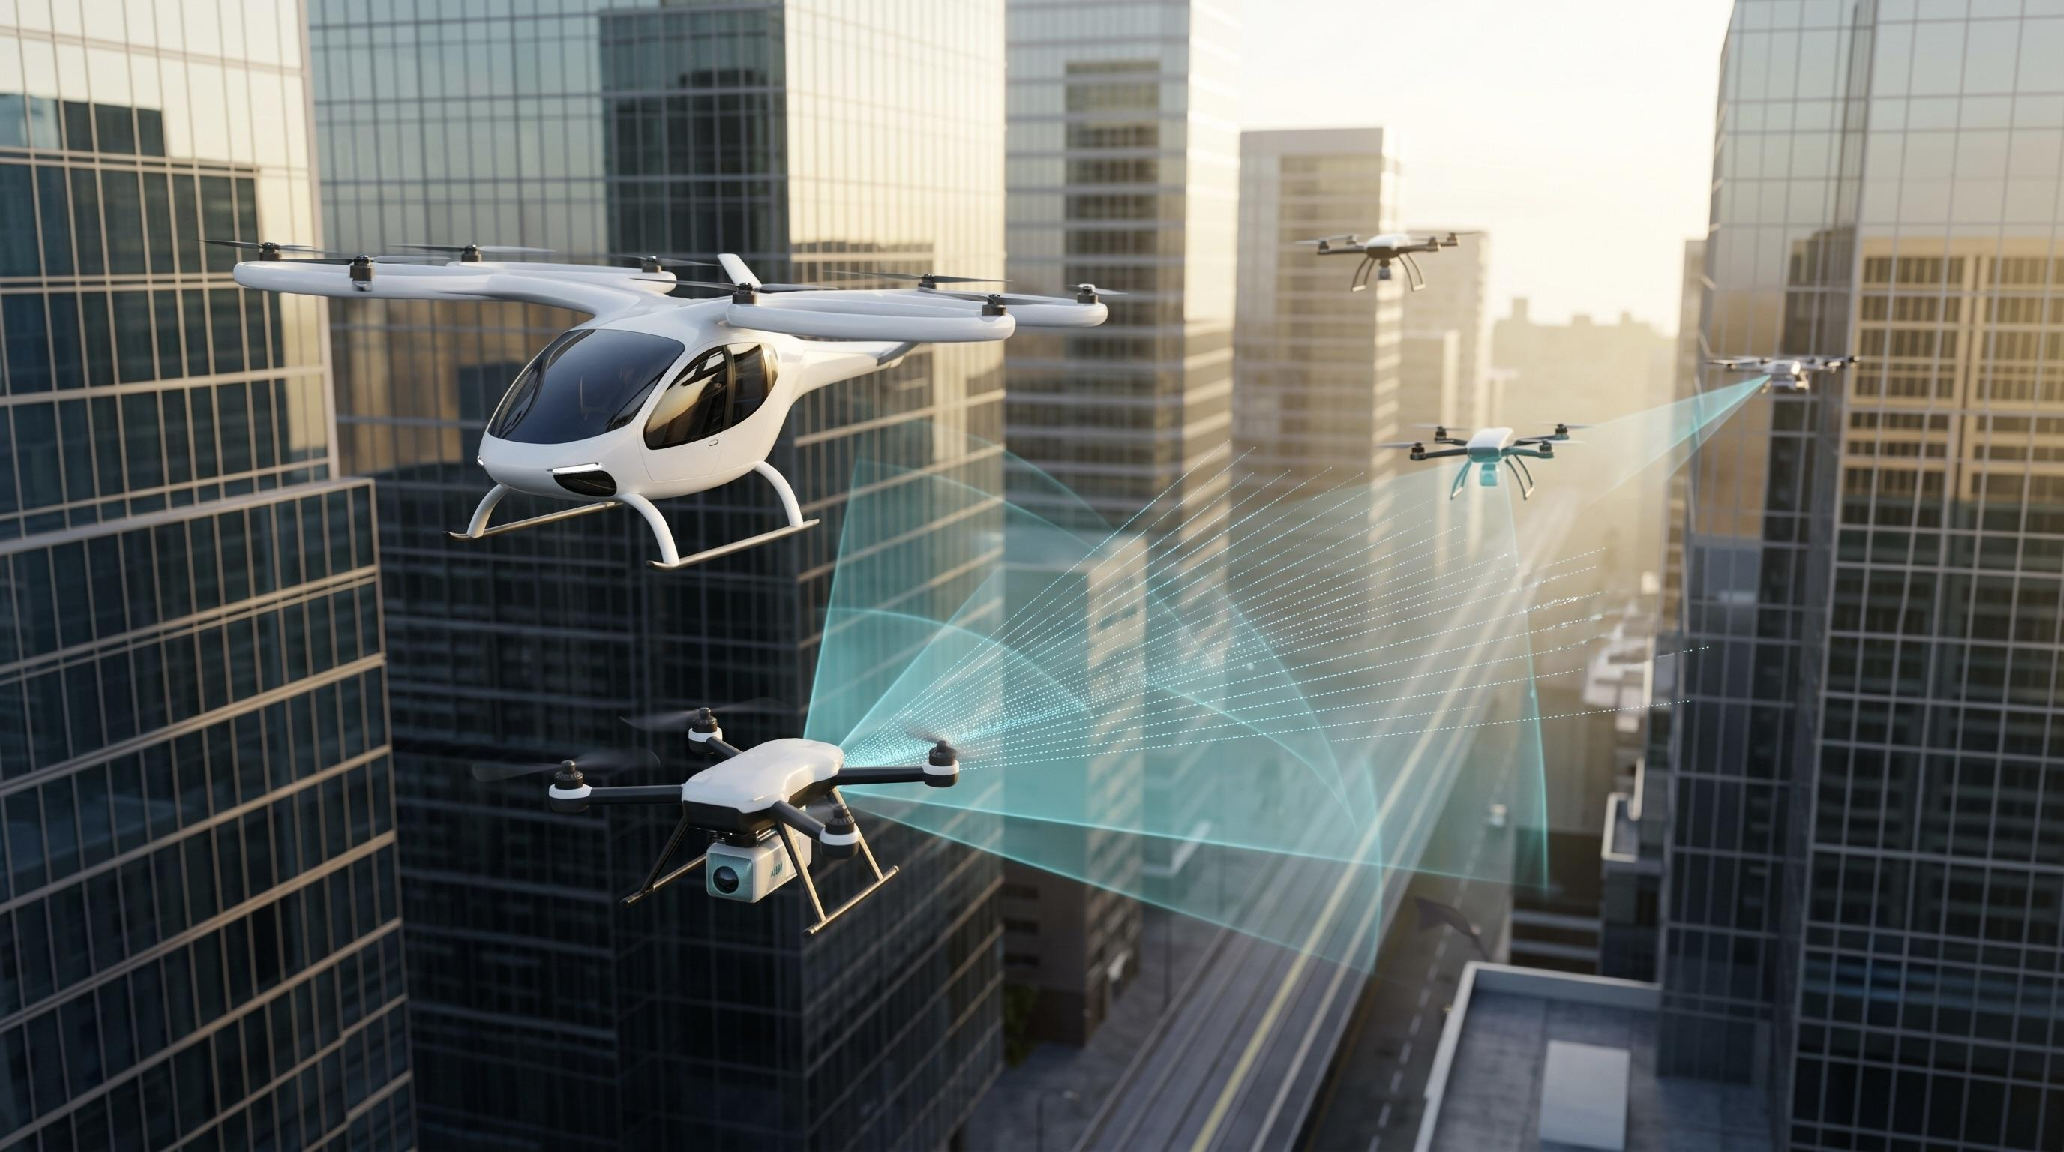
\includegraphics[width=\linewidth]{Cap1/uam_scene.pdf}
  \caption{Situational awareness for urban air mobility. An autonomous aerial
  vehicle sharing the urban canyon with other drones, manned eVTOL aircraft, and
  uncooperative traffic must perceive nearby obstacles from its onboard sensors
  (camera and point cloud) and react in real time --- the detect-and-avoid
  problem this dissertation addresses on its \emph{Sense} side.}
  \label{fig:uam_scene}
\end{figure}

This work was carried out within the FlyMov Engineering Research Center, a
partnership between the Aeronautics Institute of Technology (ITA), Embraer, and
the São Paulo Research Foundation (FAPESP), whose mission includes the
perception and decision-making technologies required for autonomous eVTOL
operation.

\subsection{Origin and Scope of the Three Studies}
\label{sec:origin}

This dissertation arose from three connected efforts that share one estimation
core and one guiding vision, yet differ in sensor, target, and setting. This
section describes how the three parts fit together.

The starting point, and the result-bearing core of the thesis, is the
range--bearing Extended Kalman Filter for tracking obstacles from a moving
platform (Chapter~\ref{cha:tracking}), developed and validated in simulation and
presented at the IEEE International Conference on Information Fusion (FUSION) in
2025 \cite{delima2025fusion}.

The second effort grew directly out of that publication. After the tracker was
presented at FUSION~2025, researchers from the UBADRON team of the Technische
Universit\"at Berlin (TU~Berlin), led by Prof.~Maarten Uijt de Haag, visited ITA.
Their team competes in the SPRIND ``Fully Autonomous Flight'' Challenge, in which
an autonomous UAV must operate without a Global Navigation Satellite System
(GNSS) and locate targets (people) on the terrain, a task with a clear
search-and-rescue motivation. They had a working
person-\emph{detection} front-end --- the early perception stage that turns raw
sensor data into per-object detections, before any tracking --- but lacked a
tracker, which is exactly what our FUSION work provided. The two groups therefore collaborated: TU~Berlin supplied
real flight data from their drones, and we adapted our estimator to their setting.
That setting is harder than the simulation: the only sensor is a single
monocular camera, so depth is unobservable and must be recovered from a
ground-plane assumption, and the platform pose is \emph{estimated} on board rather
than known, so its uncertainty must be propagated into the filter. The monocular
person tracker of Chapter~\ref{cha:monocular} is thus a distinct formulation,
linked to the FUSION tracker but adapted to a different sensor and a different
target; it was built during a three-month research stay at TU~Berlin.

The third effort addresses a different obstacle: the scarcity of annotated
three-dimensional aerial data needed to train the detection front-end of the
full camera--point-cloud pipeline. Chapter~\ref{cha:airsim} builds a synthetic
dataset in AirSim and trains and compares the detection networks on it.

The three studies are therefore distinct in their data and methods but unified by
the perception pipeline of Chapter~\ref{cha:pipeline}: \emph{one vision, three
contributions}.

\section{Detect-and-Avoid and the Sense Problem}

For any aircraft to share the airspace safely, it must be able to perceive
potential conflicts and act to prevent collisions. Aviation authorities codify
this requirement under the term \emph{Detect-and-Avoid} (D\&A), and it is a
mandatory element of the certification of autonomous and beyond-visual-line-of-sight
operations \cite{rtca2017do365}.
D\&A decomposes naturally into two coupled problems:

\begin{itemize}
  \item \textbf{Sense}, the \emph{perception} problem: detecting obstacles,
  estimating their three-dimensional position and extent, and tracking their
  motion over time from onboard sensors;
  \item \textbf{Avoid}, the \emph{decision and control} problem: planning and
  executing an evasive maneuver once a threat has been characterized.
\end{itemize}

This dissertation is concerned exclusively with the \textbf{Sense} side. The
avoidance problem (trajectory planning and control) is outside its scope and
is treated as a downstream consumer of the perception output. The essential
requirement that Sense places on Avoid goes beyond the obstacle's current
position. Avoid needs a \emph{calibrated} estimate of the obstacle's full state,
its position, velocity, and size, together with a trustworthy measure of the
uncertainty of that estimate, so that the avoidance logic can reason about
collision risk and time-to-conflict. Tracking where the obstacle \emph{is} is
therefore necessary but not sufficient. Because an evasive maneuver takes time to
plan and to fly, Avoid must reason about where the obstacle \emph{will be} several
steps ahead, and it is the perception layer that has to supply that forecast: a
track handed over without a prediction leaves the avoidance logic reacting to the
past. This is the main reason the perception output must include a temporal
tracking stage and not per-frame detections alone. The estimator developed here
supplies the forecast in the form that a recursive filter naturally affords:
its state carries position \emph{and} velocity together with a covariance, so
propagating the motion model forward yields a predicted position at any horizon,
accompanied by an uncertainty envelope that widens with that horizon. Richer
trajectory prediction, which would model the obstacle's intent rather than
extrapolate its kinematics, lies beyond the scope of this dissertation and is
taken up as future work in Chapter~\ref{cha:conclusions}. The size estimate, in
turn, bounds the spatial extent that the maneuver must clear. This emphasis on
calibrated uncertainty recurs throughout the thesis and motivates several of its
technical choices.

Within Sense, three perception sub-problems must be solved in sequence:
detection in two dimensions (locating objects in the image), detection in three
dimensions (lifting them into metric space), and tracking (maintaining their
state over time). The first two are powered by Convolutional Neural
Networks (CNNs); the third, the tracking stage, by recursive
Bayesian estimation.

\section{Problem Statement}

Concretely, we consider a UAV equipped with a camera and a source of
three-dimensional measurements (a LiDAR or a stereo/depth sensor) that must,
in real time and from a moving platform, (i) detect obstacles in its field of
view, (ii) estimate their three-dimensional position and size, and (iii) track
them over time, producing calibrated state estimates suitable for a downstream
avoidance module. Three characteristics make this difficult:

\begin{enumerate}
  \item \textbf{The observer is in motion.} Measurements are taken from a
  platform that is itself translating and rotating, so the obstacle's apparent
  motion in the sensor frame is not inertial and the sensor pose must be
  explicitly accounted for.
  \item \textbf{Sensing is noisy, and depth is hard to recover.} Every
  measurement carries noise in both range and bearing. Depth is the harder
  component: it is not \emph{directly} observable from a single monocular view,
  because the pre-image of a pixel is an entire ray, so it must be supplied either
  by an additional sensor or by an additional assumption about the scene. This is
  not to say that depth cannot be inferred from imagery at all. Modern learned
  monocular estimators do recover metric depth from a single image with useful
  accuracy \cite{bhat2023zoedepth,yang2024depthanything}, and the gap to an active
  range sensor has narrowed considerably; what remains true is that such an
  inference is indirect, and that its error is harder to characterize and to
  bound than that of a direct measurement, which matters for a certifiable
  estimator. This dissertation therefore recovers depth geometrically: from the
  point cloud where one is available (Chapters~\ref{cha:pipeline}
  and~\ref{cha:airsim}), and from a ground-plane constraint where the only sensor
  is a camera (Chapter~\ref{cha:monocular}). Even active range sensors degrade
  with distance, so the range noise is strongly range-dependent and must be modeled
  as such rather than assumed constant.
  \item \textbf{Aerial data are scarce and computational resources are limited.} Unlike ground
  autonomy, there is no abundance of annotated three-dimensional aerial
  datasets, and the perception stack must ultimately run on constrained onboard
  hardware.
\end{enumerate}

\section{Proposed Solution}
\label{sec:proposed_solution}

The approach taken here is a \emph{modular camera--point-cloud fusion pipeline},
modular in the sense that each stage exposes an explicit, low-dimensional
interface to the next and can therefore be trained, validated, and replaced
independently of the others. Figure~\ref{fig:pipeline_intro} shows the resulting
architecture end to end; it is the single artifact to which every chapter of this
dissertation contributes, and Chapter~\ref{cha:pipeline} develops it in detail.

A CNN detector first localizes objects in the image; each two-dimensional
detection is lifted into a viewing \emph{frustum} that bounds the corresponding
region of the point cloud; a point-cloud network estimates an amodal
three-dimensional bounding box (one that spans the object's full extent, including
the faces hidden from the sensor) within that frustum; and an Extended Kalman
Filter (EKF) tracks the resulting detections over time. This frustum-based
fusion follows the lineage of Frustum PointNets \cite{qi2018frustum}, adapted
here to the aerial sense-and-avoid setting.

\begin{figure}[H]
  \centering
  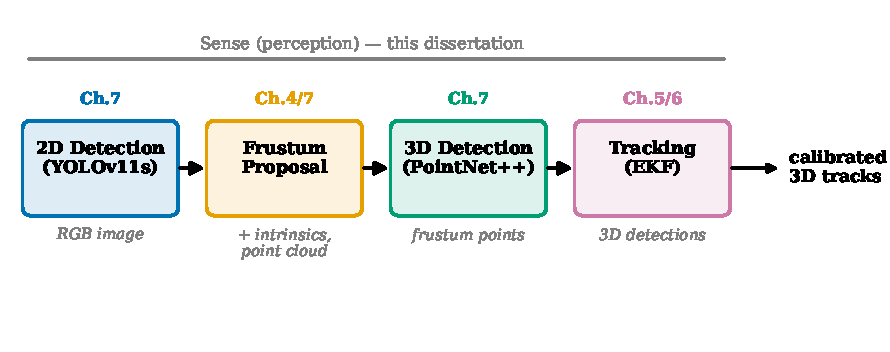
\includegraphics[width=\linewidth]{Cap4/pipeline_architecture.pdf}
  \caption{The proposed modular camera--point-cloud perception pipeline, shown
  here in overview. A 2D detector seeds a viewing frustum that crops the point
  cloud; a point-cloud network regresses a 3D box; and a recursive filter tracks
  the detections, outputting calibrated 3D tracks for the avoidance layer. Each
  of the three studies of this dissertation contributes one part of this single
  architecture, which Chapter~\ref{cha:pipeline} presents in full detail.}
  \label{fig:pipeline_intro}
\end{figure}

\subsection{Where the Point Clouds Come From}
\label{sec:cloud_provenance}

Because the pipeline consumes a point cloud at its second stage, it is worth
stating at the outset which sensor produces that cloud in each part of this work.
The three settings differ, and the distinction matters when reading the results.

\begin{itemize}
  \item In the pipeline as an \emph{architecture} (Chapter~\ref{cha:pipeline}),
  the cloud is whatever three-dimensional sensor the aircraft carries: a LiDAR, a
  stereo rig, or an RGB-D (depth) camera. The tracker consumes an abstract
  range--bearing measurement with a covariance and is indifferent to which of
  these produced it.
  \item In the simulated detection study (Chapter~\ref{cha:airsim}), the working
  cloud is produced by an \emph{idealized planar-depth camera} in AirSim, and not
  by a real LiDAR. A simulated $64$-beam LiDAR is available and is retained as an
  auxiliary channel, but at the altitudes of interest the targets are seen against
  the sky, where too few beams strike them to localize a target, whereas the dense
  depth image supplies the $10^{5}$--$3\times10^{5}$ points per frame that the
  point-cloud network needs. The idealization this entails, and its consequences
  for how the reported accuracy should be read, are stated explicitly in
  Section~\ref{sec:sensor_caveat}.
  \item In the real-flight study (Chapter~\ref{cha:monocular}) there is
  \emph{no} point cloud on the target at all. The only onboard sensor pointed at
  the person is a monocular camera, and the missing depth is recovered from a
  ground-plane constraint. A LiDAR appears in that study only offline, to survey
  the room and build the reference map against which the tracker is scored.
\end{itemize}

\section{Objectives}

The problem stated in Section~\ref{sec:proposed_solution} and the solution
sketched there translate into one overarching goal and three specific goals, one
per study. They are stated here in the order in which the dissertation pursues
them.

\subsection{General Objective}

To develop and validate the perception (\emph{Sense}) stack for UAV
detect-and-avoid in urban environments, designed as a structured modular
camera--point-cloud fusion pipeline whose tracking stage is
formulated, analyzed, and validated.

\subsection{Specific Objectives}

\begin{enumerate}
  \item To formulate the obstacle-tracking problem from a moving platform as a
  nonlinear Bayesian filtering problem, for which the EKF is the solution
  evaluated here, and to analyze
  rigorously the two natural choices of reference frame
  (global inertial versus local sensor), establishing their relationship and
  benchmarking the filter against the Cram\'er--Rao bound.
  \item To demonstrate the generality of the resulting framework by adapting it
  to monocular person tracking from a real UAV, explicitly propagating the
  camera-pose uncertainty into the estimator.
  \item To design the detection front-end of the pipeline, that is, the
  two- and three-dimensional detection stages that produce the measurements the
  tracker consumes, and to assemble a fully-annotated synthetic aerial dataset
  that enables its training in the absence of large-scale real data, and to
  evaluate the front-end, together with alternative detection paradigms, on a
  moving-observer campaign with three-dimensional detection and tracking metrics.
\end{enumerate}

\section{Contributions}

The dissertation makes the following contributions, organized as one overarching
system, the perception pipeline, and three self-contained studies that
realize and validate its components:

\begin{enumerate}
  \item \textbf{A rigorous treatment of EKF tracking from a moving platform}
  (Chapter~\ref{cha:tracking}). We give a unified derivation of the global- and
  local-frame formulations for spherical (range--bearing) measurements, prove
  that the two are \emph{mathematically equivalent} under a known platform pose
  and isotropic process noise, and characterize precisely the conditions under
  which they genuinely diverge. The formulation was presented at the IEEE
  International Conference on Information Fusion \cite{delima2025fusion}.
  \item \textbf{Generality of the framework, validated on real data}
  (Chapter~\ref{cha:monocular}). During a three-month research stay with the
  UBADRON team at the Technische Universit\"at Berlin (TU Berlin), the
  same estimator was extended to monocular person tracking from a UAV, where the
  platform pose is uncertain and depth is unobservable. A person detector trained on a union of
  complementary aerial datasets (spanning urban, rural near-range, and
  high-altitude regimes) supplies the image measurements; a ground-plane
  constraint recovers metric position from the single view; and the filter
  propagates the six-degree-of-freedom camera-pose covariance into its
  innovation, which an ablation shows to be necessary for statistical
  consistency under aggressive platform motion. The system is validated on real
  flights against a LiDAR-referenced ground truth.
  \item \textbf{A synthetic aerial dataset and detection front-end}
  (Chapter~\ref{cha:airsim}). A configurable, fully-annotated dataset built in
  AirSim addresses the scarcity of three-dimensional aerial data: a pixel-exact
  synthetic-composition scheme circumvents the simulator's unreliable annotation
  interfaces, and a geometric construction supplies trustworthy 3D boxes. The data
  are employed to train the CNN-based two- and three-dimensional detectors, which
  are then evaluated on a moving-observer campaign with the standard
  multi-object-tracking metrics of autonomous driving. The study further identifies
  foreground extraction, rather than the box regressor, as the dominant factor in 3D
  localization accuracy, and provides the first empirical comparison of the
  two-stage frustum design against the single-stage voxel paradigm on aerial data.
  \item \textbf{A systematic literature review} (Chapter~\ref{cha:relatedwork})
  following the PRISMA, Kitchenham, and Wohlin methodologies, which establishes
  that frustum-based camera--point-cloud detection has not previously been
  brought to UAV sense-and-avoid, and locates this work within that gap.
\end{enumerate}

\section{Publications}

The tracking formulation of Chapter~\ref{cha:tracking} was published as:
de~Lima, Dias, and Maximo, \emph{Extended Kalman Filter-Based Object Tracking
Using Global and Local Frames}, IEEE International Conference on Information
Fusion (FUSION), 2025 \cite{delima2025fusion}. The real-data study of
Chapter~\ref{cha:monocular}, developed with the UBADRON team of the Chair of
Flight Guidance and Air Transport at TU~Berlin, is in preparation for publication.

\section{Outline of the Dissertation}

The remainder of the dissertation is organized so that a shared foundation
supports three self-contained studies. Chapter~\ref{cha:background} establishes
the common theoretical framework, comprising recursive Bayesian estimation and the
EKF, coordinate frames, motion and measurement models, consistency metrics, and the
neural-network building blocks from which every later chapter draws.
Chapter~\ref{cha:relatedwork} reviews the literature and substantiates the
research gap. Chapter~\ref{cha:pipeline} presents the perception pipeline as a
single architecture and shows how the three studies map onto it. The three study
chapters then follow, each self-contained with its own methodology and results:
Chapter~\ref{cha:tracking} develops and analyzes the EKF tracker in global and
local frames; Chapter~\ref{cha:monocular} extends it to monocular tracking from a
real UAV; and Chapter~\ref{cha:airsim} builds the synthetic dataset and the
detection front-end. Chapter~\ref{cha:conclusions} synthesizes the three studies,
revisits the contributions, and outlines future work toward an integrated,
onboard sense-and-avoid system.

\section{Note on the Use of Artificial-Intelligence Tools}
\label{sec:ai_disclaimer}

In the interest of transparency, the author discloses the use of
Artificial-Intelligence (AI) assistants during the preparation of this
dissertation. AI-based tools (large language models) were used as a writing aid,
to improve the clarity, grammar, and flow of the English text, to help structure
and format \LaTeX{} and to assist with routine plotting and figure-generation
code. They were \emph{not} used to produce experimental results: every model,
derivation, experiment, dataset, and numerical result reported here was designed,
implemented, executed, and verified by the author. All technical claims were
checked against the underlying data and code, and the author takes full
responsibility for the content.


\chapter{Theoretical Background}\label{cha:background}
% =====================================================================
% Chapter 2 --- Theoretical Background                        [cross-cutting]
% Establishes ONCE the shared framework used by all later chapters, fixing
% the notation reused verbatim in Chapters 5--7. Two pillars: recursive
% Bayesian estimation (the tracker) and deep networks (the detector).
% =====================================================================

This chapter introduces the mathematical tools used throughout the dissertation
and fixes the notation reused in the later chapters. It rests on two pillars:
recursive Bayesian estimation, which underpins the tracking stage
(Chapters~\ref{cha:tracking} and \ref{cha:monocular}), and convolutional neural
networks, which underpin the detection front-end (Chapters~\ref{cha:pipeline}
and \ref{cha:airsim}). The treatment is deliberately self-contained but assumes
familiarity with linear algebra and probability.

\section{Bayesian Recursive Estimation and the Kalman Filter}

The tracking problem is an instance of \emph{recursive state estimation}: an
unobserved state evolves in time and is observed only through noisy
measurements. We model it by the discrete-time, possibly nonlinear, state-space
system
\begin{align}
  \bm{x}_k &= \bm{f}(\bm{x}_{k-1}) + \bm{w}_{k-1}, & \bm{w}_{k-1} &\sim \mathcal{N}(\bm{0},\bm{Q}_{k-1}), \label{eq:ss_process}\\
  \bm{z}_k &= \bm{h}(\bm{x}_k) + \bm{v}_k,         & \bm{v}_k     &\sim \mathcal{N}(\bm{0},\bm{R}_k),     \label{eq:ss_meas}
\end{align}
where $\bm{x}_k$ is the state, $\bm{z}_k$ the measurement, $\bm{f}(\cdot)$ the
process model, $\bm{h}(\cdot)$ the measurement model, and $\bm{w}_k,\bm{v}_k$
mutually independent zero-mean Gaussian process and measurement noises. The state
is assumed Markovian and the measurements conditionally independent given the
state.

Bayesian filtering propagates the posterior density $p(\bm{x}_k\mid \bm{z}_{1:k})$
in two alternating steps: a \emph{prediction} that pushes the previous posterior
through the process model (the Chapman--Kolmogorov equation), and an
\emph{update} that fuses the new measurement through Bayes' rule. For the
linear-Gaussian special case, with $\bm{f}(\bm{x})=\bm{F}\bm{x}$ and
$\bm{h}(\bm{x})=\bm{H}\bm{x}$, these integrals admit a closed form, the
\emph{Kalman filter} (KF) \cite{barshalom2001,brookner1998}: the posterior
remains Gaussian and is summarized by its mean $\hat{\bm{x}}_{k|k}$ and covariance
$\bm{P}_{k|k}$, propagated by
\begin{align}
  \hat{\bm{x}}_{k|k-1} &= \bm{F}\,\hat{\bm{x}}_{k-1|k-1}, &
  \bm{P}_{k|k-1} &= \bm{F}\,\bm{P}_{k-1|k-1}\,\bm{F}^{\top} + \bm{Q}, \label{eq:kf_predict}\\
  \bm{K}_k &= \bm{P}_{k|k-1}\bm{H}^{\top}\bm{S}_k^{-1}, &
  \bm{S}_k &= \bm{H}\,\bm{P}_{k|k-1}\,\bm{H}^{\top} + \bm{R}, \label{eq:kf_gain}\\
  \hat{\bm{x}}_{k|k} &= \hat{\bm{x}}_{k|k-1} + \bm{K}_k\bm{\nu}_k, &
  \bm{P}_{k|k} &= (\bm{I}-\bm{K}_k\bm{H})\,\bm{P}_{k|k-1}, \label{eq:kf_update}
\end{align}
with innovation $\bm{\nu}_k=\bm{z}_k-\bm{H}\hat{\bm{x}}_{k|k-1}$. The KF is the
optimal (minimum mean-square-error) estimator in the linear-Gaussian case.

\section{The Extended Kalman Filter}

The tracking models of this work are nonlinear, since the platform rotates and the
measurements are spherical or projective, so the linear KF does not apply
directly. The Extended Kalman Filter (EKF) retains the Gaussian parameterization
but linearizes the nonlinear models about the current estimate
\cite{terejanu2008,barshalom2001}.

\subsection{Linearization}

Let
\begin{equation}
  \bm{F}_k = \left.\frac{\partial \bm{f}(\bm{x})}{\partial \bm{x}}\right|_{\bm{x}=\hat{\bm{x}}_{k-1|k-1}},
  \qquad \mbox{and} \qquad
  \bm{H}_k = \left.\frac{\partial \bm{h}(\bm{x})}{\partial \bm{x}}\right|_{\bm{x}=\hat{\bm{x}}_{k|k-1}}
  \label{eq:ekf_jac}
\end{equation}
be the Jacobians of the process and measurement models evaluated at the predicted
state. The EKF propagates the covariance through these first-order
approximations.

\subsection{Prediction and Update}

The EKF's recursion mirrors \eqref{eq:kf_predict}--\eqref{eq:kf_update}, with the
nonlinear models used for the means and their Jacobians for the covariances:
\begin{align}
  \hat{\bm{x}}_{k|k-1} &= \bm{f}(\hat{\bm{x}}_{k-1|k-1}), &
  \bm{P}_{k|k-1} &= \bm{F}_k\,\bm{P}_{k-1|k-1}\,\bm{F}_k^{\top} + \bm{Q}, \label{eq:ekf_predict}\\
  \bm{\nu}_k &= \bm{z}_k - \bm{h}(\hat{\bm{x}}_{k|k-1}), &
  \bm{S}_k &= \bm{H}_k\,\bm{P}_{k|k-1}\,\bm{H}_k^{\top} + \bm{R}_k, \label{eq:ekf_innov}\\
  \bm{K}_k &= \bm{P}_{k|k-1}\bm{H}_k^{\top}\bm{S}_k^{-1}, &
  \hat{\bm{x}}_{k|k} &= \hat{\bm{x}}_{k|k-1} + \bm{K}_k\bm{\nu}_k, \label{eq:ekf_gain}
\end{align}
and $\bm{P}_{k|k} = (\bm{I}-\bm{K}_k\bm{H}_k)\,\bm{P}_{k|k-1}$. Unlike the linear
KF, the EKF is neither optimal nor unbiased: the linearization
\eqref{eq:ekf_jac} discards higher-order terms, and the magnitude of the
resulting error depends on how nonlinear the process and measurement models are
over the support of the state covariance. This caveat matters in Chapter~\ref{cha:tracking}, where two
algebraically distinct EKF formulations are compared.

\section{Coordinate Frames and Rigid-Body Transformations}

\subsection{World, Body, and Optical Frames}

Three right-handed frames are used. The \emph{world} frame $\mathcal{W}$ is a
local inertial East--North--Up (ENU) frame fixed to the operating area. The
\emph{body} frame $\mathcal{B}$ is attached to the platform (Forward--Left--Up).
The \emph{optical} frame $\mathcal{O}$ is attached to the camera (the computer
vision convention: $x$ right, $y$ down, $z$ forward). Estimation is carried in
$\mathcal{W}$ or $\mathcal{B}$ depending on the formulation, while measurements
originate in $\mathcal{O}$.

\subsection{Rotations, Euler Angles, and Homogeneous Transforms}

A rotation is an element of $SO(3)$, represented here by a $3\times3$ matrix
$\bm{R}$ with $\bm{R}^{\top}\bm{R}=\bm{I}$ and $\det\bm{R}=1$. Using the
$Z$--$Y$--$X$ (yaw--pitch--roll) Euler convention adopted throughout,
\begin{equation}
  \bm{R}(\phi,\theta,\psi) = \bm{R}_z(\psi)\,\bm{R}_y(\theta)\,\bm{R}_x(\phi),
  \label{eq:euler}
\end{equation}
with the elementary rotations
\begin{equation}
  \bm{R}_x(\phi)=\!\begin{bmatrix}1&0&0\\0&c_\phi&-s_\phi\\0&s_\phi&c_\phi\end{bmatrix}\!,\;
  \bm{R}_y(\theta)=\!\begin{bmatrix}c_\theta&0&s_\theta\\0&1&0\\-s_\theta&0&c_\theta\end{bmatrix}\!,\;
  \bm{R}_z(\psi)=\!\begin{bmatrix}c_\psi&-s_\psi&0\\s_\psi&c_\psi&0\\0&0&1\end{bmatrix}\!,
  \label{eq:elementary}
\end{equation}
where $c_\bullet=\cos$ and $s_\bullet=\sin$. With this convention $\bm{R}$ maps
body coordinates to world coordinates, and a point transforms as
$\bm{p}^{\mathcal{W}}=\bm{R}\,\bm{p}^{\mathcal{B}}+\bm{t}$; the inverse map is
$\bm{p}^{\mathcal{B}}=\bm{R}^{\top}(\bm{p}^{\mathcal{W}}-\bm{t})$. Equivalently, in
homogeneous coordinates,
\begin{equation}
  \begin{bmatrix} \bm{p}^{\mathcal{W}} \\ 1 \end{bmatrix}
  = \underbrace{\begin{bmatrix} \bm{R} & \bm{t} \\ \bm{0} & 1 \end{bmatrix}}_{\bm{T}\,\in\, SE(3)}
    \begin{bmatrix} \bm{p}^{\mathcal{B}} \\ 1 \end{bmatrix},
  \label{eq:se3_transform}
\end{equation}
which compactly writes the world point as a function of the body point through the
pose $\bm{T}\in SE(3)$.

\subsection{Pose Perturbations}

When the platform pose is uncertain (Chapter~\ref{cha:monocular}), its
uncertainty must be propagated through the geometry. A small pose perturbation is
represented in the tangent space of $SE(3)$ by a six-vector
$\bm{\xi}=[\bm{\delta\theta}^{\top}\;\bm{\delta t}^{\top}]^{\top}$, and to first
order a point in the camera frame perturbs as
\begin{equation}
  \delta\bm{p}^{\mathcal{O}} \approx -[\bm{p}^{\mathcal{O}}]_\times\,\bm{\delta\theta} + \bm{\delta t},
  \qquad
  [\bm{a}]_\times = \begin{bmatrix} 0 & -a_3 & a_2 \\ a_3 & 0 & -a_1 \\ -a_2 & a_1 & 0 \end{bmatrix},
  \label{eq:se3_pert}
\end{equation}
where $[\,\cdot\,]_\times$ is the skew-symmetric (cross-product) matrix
\cite{sola2018microlie}. This linearization is the basis of the extrinsic
Jacobian derived in Chapter~\ref{cha:monocular}.

\section{Motion Models}

\subsection{Constant-Velocity and Constant-Acceleration Models}

In the absence of a control input, target motion is described by a kinematic
model. The \emph{constant-velocity} (CV) model assumes piecewise-constant
velocity perturbed by random accelerations; per Cartesian axis, the
position--velocity pair $(p,\dot p)$ propagates as
\begin{equation}
  \begin{bmatrix} p_{k+1} \\ \dot p_{k+1} \end{bmatrix}
  = \begin{bmatrix} 1 & \Delta t \\ 0 & 1 \end{bmatrix}
    \begin{bmatrix} p_{k} \\ \dot p_{k} \end{bmatrix} + \text{noise},
  \label{eq:cv}
\end{equation}
with sampling interval $\Delta t$. The \emph{constant-acceleration} model adds an
explicit acceleration state. This work uses the CV model, with acceleration
represented as process noise rather than as a state variable.

\subsection{Process Noise}

Modelling the unknown acceleration as a continuous white noise of intensity
$\sigma_a^2$ yields, after discretization, the per-axis process-noise covariance
\begin{equation}
  \bm{Q}_{\text{axis}} = \sigma_a^{2}
  \begin{bmatrix} \Delta t^{3}/3 & \Delta t^{2}/2 \\[2pt] \Delta t^{2}/2 & \Delta t \end{bmatrix}.
  \label{eq:cwna}
\end{equation}
When the same intensity $\sigma_a$ is used on all axes, the resulting block-diagonal
$\bm{Q}$ is invariant under rotation of the coordinate axes, a property that has
a decisive consequence in Chapter~\ref{cha:tracking}.

\section{Measurement Models}

\subsection{Range--Bearing (Spherical) Measurements}

A depth or fused camera--LiDAR sensor reports the relative position of a target in
spherical coordinates. Writing the relative position in the sensor frame as
$\bm{p}^{c}=[x^{c},y^{c},z^{c}]^{\top}$, the measurement comprises range, azimuth
and elevation,
\begin{equation}
  \rho = \lVert\bm{p}^{c}\rVert,\quad
  \alpha = \operatorname{atan2}(y^{c},x^{c}),\quad
  \beta = \operatorname{atan2}\!\big(z^{c},\sqrt{(x^{c})^2+(y^{c})^2}\big).
  \label{eq:spherical}
\end{equation}
Ranging accuracy degrades with distance, which is captured by a heteroscedastic
range variance $\sigma_\rho^2 = \alpha_\rho\,\rho^2$, with $\alpha_\rho$ a
sensor-dependent coefficient \cite{fernandes2020}. This model is used by the
trackers of Chapters~\ref{cha:tracking}.

\subsection{Pinhole Projection and Lens Distortion}

A monocular camera (Chapter~\ref{cha:monocular}) instead measures the
\emph{pixel} projection of a world point. Under the pinhole model, a point
$\bm{X}^{\mathcal{O}}=[X,Y,Z]^{\top}$ in the optical frame projects to
\begin{equation}
  \bm{u} = \pi\!\big(\bm{K}\,\bm{X}^{\mathcal{O}}\big),
  \qquad
  \pi\!\left(\begin{bmatrix}X\\Y\\Z\end{bmatrix}\right) = \begin{bmatrix}X/Z\\Y/Z\end{bmatrix},
  \qquad
  \bm{K}=\begin{bmatrix} f_x & 0 & c_x \\ 0 & f_y & c_y \\ 0 & 0 & 1 \end{bmatrix},
  \label{eq:pinhole}
\end{equation}
where $\bm{K}$ is the intrinsic matrix ($f_x,f_y$ focal lengths, $(c_x,c_y)$
principal point). Real lenses introduce radial and tangential (plumb-bob)
distortion, parameterized by coefficients $(k_1,k_2,k_3,p_1,p_2)$, which must be
removed from each pixel measurement before it enters the filter; the procedure is
detailed in Chapter~\ref{cha:monocular}.

\section{Performance and Consistency Metrics}

Several families of metrics are used across the dissertation: the first three
evaluate the estimator, in terms of tracking accuracy, consistency, and
optimality, and the last evaluates the detection and tracking chain.

\subsection{Accuracy}
The root-mean-square error (RMSE) of the position estimate,
averaged over $M$ Monte~Carlo runs, summarizes accuracy:
\begin{equation}
  \mathrm{RMSE}(k)=\left(\frac1M\sum_{i=1}^{M}\big\lVert \bm{p}_k^{(i)}-\hat{\bm{p}}_k^{(i)}\big\rVert^2\right)^{1/2}.
  \label{eq:rmse}
\end{equation}

\subsection{Consistency}
A filter is \emph{consistent} when its reported
covariance matches its actual error. With ground truth available, the normalized
estimation error squared (NEES) of an $n$-dimensional state,
\begin{equation}
  \epsilon_k = (\bm{x}_k-\hat{\bm{x}}_{k|k})^{\top}\,\bm{P}_{k|k}^{-1}\,(\bm{x}_k-\hat{\bm{x}}_{k|k}),
  \label{eq:nees}
\end{equation}
follows a $\chi^2_n$ distribution (mean $n$) for a consistent filter. When ground
truth is unavailable, the normalized innovation squared (NIS),
$\eta_k=\bm{\nu}_k^{\top}\bm{S}_k^{-1}\bm{\nu}_k\sim\chi^2_m$ for $m$-dimensional
measurements, provides an analogous, measurement-only check \cite{barshalom2001}.

\subsection{Optimality Bound}
The posterior Cram\'er--Rao bound (PCRB) lower-bounds
the achievable estimation-error covariance. For the filtering problem it is
obtained from the Fisher information recursion
\begin{equation}
  \bm{J}_{k+1} = \big(\bm{Q}+\bm{F}\bm{J}_k^{-1}\bm{F}^{\top}\big)^{-1}
              + \mathbb{E}\!\big[\bm{H}_{k+1}^{\top}\bm{R}_{k+1}^{-1}\bm{H}_{k+1}\big],
  \label{eq:pcrb}
\end{equation}
where $\bm{J}_k$ is the Fisher information matrix. Its inverse lower-bounds the
estimation-error covariance of any unbiased estimator,
$\mathbb{E}[(\bm{x}_k-\hat{\bm{x}}_k)(\bm{x}_k-\hat{\bm{x}}_k)^{\top}]\succeq\bm{J}_k^{-1}$,
so the diagonal of $\bm{J}_k^{-1}$ bounds the per-component error variance from
below \cite{tichavsky1998}. This bound is used to assess near-optimality of the
tracker in Chapter~\ref{cha:tracking}.

\subsection{Detection and Multi-Object-Tracking Metrics}
\label{sec:detmetrics}

The detection front-end (Chapter~\ref{cha:airsim}) is evaluated with the standard
detection and tracking measures. A detection that matches a ground-truth object
under an overlap or distance gate is a true positive (TP) and otherwise a false
positive (FP); a ground-truth object with no matching detection is a false
negative (FN). \emph{Precision} ($P$), \emph{recall} ($R$), and their harmonic
mean $F_1$ are then
\begin{equation}
  P = \frac{\mathrm{TP}}{\mathrm{TP}+\mathrm{FP}}, \qquad
  R = \frac{\mathrm{TP}}{\mathrm{TP}+\mathrm{FN}}, \qquad
  F_1 = \frac{2\,P\,R}{P+R}.
  \label{eq:prf1}
\end{equation}
Sweeping the detector's confidence threshold traces a precision--recall curve
whose area is the average precision; averaging it over classes and overlap gates
gives the mean average precision (mAP), as standardized by the COCO benchmark
\cite{lin2014coco}.
For the temporal chain, multi-object-tracking accuracy (MOTA) aggregates false positives,
misses, and identity switches at one operating point, and the identity score
(IDF1) measures how consistently tracks preserve object identity. Because MOTA is
read at a single threshold, the driving community favors its integral over recall,
the average MOTA (AMOTA) \cite{weng2020ab3dmot}, which characterizes the
detector--tracker chain independently of a particular threshold; its companion
AMOTP averages the localization error of matched tracks. These measures are used
throughout Chapter~\ref{cha:airsim}.

\section{Deep Learning for Perception}

The detection front-end of the pipeline is built from neural networks; this
section summarizes the building blocks used in Chapters~\ref{cha:pipeline} and
\ref{cha:airsim}.

\subsection{Convolutional Neural Networks}

A convolutional neural network (CNN) applies learned convolutional filters across
an image, sharing weights spatially and stacking layers to build a hierarchy of
features, from edges and textures to object parts and whole objects. Weight
sharing makes CNNs parameter-efficient and translation-equivariant, which is why
they are the standard tool for image perception \cite{lecun2015deeplearning}.

\subsection{Two-Dimensional Object Detection and the YOLO Family}

Object detection localizes and classifies objects within an image. The decisive
split is between \emph{two-stage} detectors, such as the R-CNN family, which first
propose candidate regions and then classify and refine each one, and
\emph{one-stage} detectors, which predict all boxes and class scores in a single
forward pass. The You Only Look Once (YOLO) detector \cite{redmon2016yolo}
introduced the one-stage idea: the image is processed once by a fully
convolutional network that, over a dense spatial grid, directly regresses box
coordinates, an objectness score, and class probabilities. Removing the separate
proposal stage is what gives YOLO its real-time throughput, which is the property
that an onboard aerial system needs.

Architecturally, a modern YOLO network has three parts. A \emph{backbone} (a deep
convolutional feature extractor, in recent versions built from cross-stage-partial
blocks that split and merge feature maps to cut redundant computation) produces a
hierarchy of feature maps. A \emph{neck} (a feature-pyramid / path-aggregation
network) fuses these maps across scales so that both small and large objects are
represented. A \emph{detection head} then emits the dense predictions. Relative to
the original detector, the versions used today (the Ultralytics
YOLOv8--YOLOv11 line \cite{ultralytics2024yolo11}) introduce three changes that
matter for small aerial targets: they are \emph{anchor-free}, predicting box
offsets directly from grid locations instead of from hand-designed anchor boxes;
they use \emph{decoupled heads}, separating the classification and box-regression
branches; and they insert lightweight \emph{attention} modules in the backbone,
which reweight feature channels and spatial locations and improve the detection of
small, low-contrast objects, while preserving the single-pass design. A practical
difficulty in the aerial setting is \emph{domain shift}: because a detector's
accuracy depends on the match between its training distribution and the deployment
scene, a network meant to operate in an unseen environment is commonly trained on
a diverse union of datasets to widen its operating envelope.

\subsection{Point-Cloud Processing: PointNet and PointNet\texttt{++}}

Three-dimensional detection operates on point clouds, an \emph{unordered} set of
$N$ points $\{\bm{p}_i\in\mathbb{R}^3\}$ with no grid structure, so the convolution
that underpins image CNNs does not apply. PointNet \cite{qi2017pointnet} resolves
this with a construction that is invariant to the ordering of the points: each
point is passed independently through a \emph{shared} multilayer perceptron
$h(\cdot)$, and the resulting per-point features are aggregated by a
\emph{symmetric} function, max-pooling, into a single global descriptor
$\bm{g}=\max_i h(\bm{p}_i)$. Because max-pooling does not depend on the order of
its inputs, the network is permutation-invariant by construction; an optional
learned input alignment (a small ``T-Net'' that regresses a transformation
matrix) further canonicalizes the pose of the cloud. The limitation of this design
is that a single global pooling captures the overall shape but discards
\emph{local} neighborhood structure, which matters for fine geometry.

PointNet\texttt{++} \cite{qi2017pointnetpp} removes that limitation by applying
PointNet \emph{hierarchically}. Each \emph{set-abstraction} level (i) samples a
subset of centroid points by farthest-point sampling, (ii) groups the neighbors of
each centroid within a query radius (a ``ball query''), and (iii) encodes each
local group with a small PointNet. Stacking several such levels yields a
progressively coarser set of points carrying progressively richer local features,
so the network learns geometry at multiple scales, much as a CNN does on images.
This hierarchical point-set encoder is the workhorse of the 3D detector built in
this work. Frustum PointNets \cite{qi2018frustum} fuse it with the 2D detector:
each image detection defines a viewing frustum that crops the point cloud to a
small candidate region, and a PointNet\texttt{++} regresses the amodal 3D box
within that frustum, fusing the two modalities by geometry rather than in a learned
latent space.

\subsection{Single-Stage Voxel Detection}

The frustum approach is a \emph{two-stage} detector: a 2D network proposes
regions and a point-cloud network refines them in 3D, so its recall is bounded by
the 2D stage. The complementary \emph{single-stage} family detects directly in
the point cloud over the whole scene. Because raw points are irregular, these
methods first impose a regular structure: VoxelNet and the SECOND network
\cite{yan2018second} (a method name) quantize space into 3D voxels and apply (sparse) 3D
convolutions, while PointPillars \cite{lang2019pointpillars} collapses the
vertical axis into a bird's-eye-view (BEV) grid of \emph{pillars}, encodes each
pillar with a small PointNet, and runs an ordinary 2D convolutional backbone on
the resulting pseudo-image, trading a little vertical resolution for real-time
speed. Detection heads are increasingly \emph{center-based}: rather than
classifying anchor boxes, the network predicts a heatmap whose peaks are object
centers and regresses the box parameters at each peak \cite{zhou2019objects}.
This single-stage voxel paradigm is not part of the proposed pipeline; it is
included as the comparison baseline against which the two-stage frustum design is
evaluated on aerial data in Chapter~\ref{cha:airsim}.

\subsection{Training Losses for Detection}

Detectors are dominated by background: the vast majority of candidate locations
contain no object. Trained naively, the classifier is overwhelmed by easy
negatives. The \emph{focal loss} \cite{lin2017focal} addresses this by
down-weighting well-classified examples,
$\mathrm{FL}(p_t)=-\alpha_t\,(1-p_t)^{\gamma}\log p_t$, where $p_t$ is the
predicted probability of the true class and $\gamma>0$ concentrates the gradient
on hard examples. It is well suited to the objectness and heatmap classification
heads of dense detectors, whereas the continuous box parameters (center and size)
are regressed with a smooth-$L_1$ (Huber) loss.


\chapter{Related Work and Research Gap}\label{cha:relatedwork}
% =====================================================================
% Chapter 3 --- Related Work and Research Gap                 [cross-cutting]
% Based on the author's systematic literature review (DEFESA SLR):
% PRISMA 2020 + Kitchenham 5-criterion QA + Wohlin snowballing.
% Centrepiece: the uniqueness matrix and the "why nobody did this" argument.
% =====================================================================

This chapter surveys the literature relevant to the perception pipeline of
Chapter~\ref{cha:pipeline} and establishes the gap that the dissertation fills.
Rather than an ad-hoc narrative, the review follows a systematic protocol, whose
methodology is described first; the body of work is then organised thematically,
and the chapter closes by making the gap explicit and arguing why it has remained
open.

\section{Review Methodology}

\subsection{Protocol and Research Question}

The review follows the PRISMA~2020 reporting guideline \cite{page2021prisma},
the quality-assessment practice of Kitchenham and Charters
\cite{kitchenham2007slr}, and the snowballing guidelines of Wohlin
\cite{wohlin2014snowball}. It is driven by a single research question, framed in
the PICOC form:

\begin{quote}
\emph{Which CNN-based techniques have been applied for situational-awareness
perception (sense) of autonomous aerial vehicles in urban environments, using
camera and point-cloud fusion for 3D object detection and tracking?}
\end{quote}

The \emph{population} is autonomous aerial vehicles in urban environments; the
\emph{intervention} is CNN-based pipelines combining 2D detection with
point-cloud processing; the \emph{comparison} baselines are monocular, stereo,
and LiDAR-only methods; the \emph{outcome} is 3D detection and tracking accuracy
with real-time feasibility; and the \emph{context} is urban sense-and-avoid
(perception only).

\subsection{Sources, Search, and Selection}

Automated searches of OpenAlex, Semantic Scholar, and academic web search
engines were run with three query families --- (i) UAV sense-and-avoid with deep
perception, (ii) frustum- and PointNet-based 3D detection, and (iii)
LiDAR--camera fusion for aerial 3D detection --- and complemented by backward and
forward snowballing (one-hop) from four seed papers: PointNet
\cite{qi2017pointnet}, Frustum PointNets \cite{qi2018frustum}, the UAV3D
benchmark \cite{ye2024uav3d}, and a recent UAV 3D-perception survey. Studies were
included if published in 2017--2026 (the year PointNet appeared), addressing
perception (detection, tracking, or situational awareness) for UAVs or for
ground-vehicle techniques transferable to UAVs, and containing a deep-learning
component; works addressing only avoidance, planning, or control, lacking a
learning component, or in unrelated domains were excluded. Each retained study
was scored on the five Kitchenham criteria of Table~\ref{tab:qa}, on a
$0$/$0.5$/$1$ scale; following the protocol, studies scoring below $2.5$ were
demoted to background text and excluded from the synthesis. The process was
managed with Rayyan, Zotero, and Parsifal.

\begin{table}[H]
  \centering
  \caption{Quality-assessment criteria (Kitchenham), each scored $0$/$0.5$/$1$.}
  \label{tab:qa}
  \begin{tabular}{@{}cl@{}}
    \toprule
    Criterion & Question \\
    \midrule
    Q1 & Are the problem and objectives clearly stated? \\
    Q2 & Is the methodology described in enough detail to reproduce? \\
    Q3 & Are there quantitative experiments on an established benchmark? \\
    Q4 & Does the work address a component of the proposed pipeline? \\
    Q5 & Is the contribution clearly differentiated from prior art? \\
    \bottomrule
  \end{tabular}
\end{table}

\subsection{Outcome of the Search}

The automated searches returned roughly $150$ records; five thematic
gap-filling searches added $50$; and snowballing added $44$, for $244$ records
in total. After de-duplication, $183$ unique records remained. Title-and-abstract
screening retained $174$ studies (with $7$ deferred to full-text assessment and
$2$ cross-snowball duplicates removed). Quality assessment passed $173$ studies
(mean score $4.05/5$, median $4.5$; $51\%$ from top-tier venues); a single survey
fell below the cut-off and was demoted to background. These $173$ studies form
the basis of the synthesis that follows.

\section{Two-Dimensional Detection for Aerial Imagery}

The pipeline's first stage is a 2D detector. The one-stage YOLO family
\cite{redmon2016yolo}, which regresses bounding boxes and class scores in a
single pass, dominates aerial detection because of its real-time throughput; a
substantial body of work adapts it to the small objects, oblique viewpoints, and
scale variation characteristic of aerial imagery. These detectors are mature and
are treated here as a reliable building block rather than a research
contribution of this work.

\section{Frustum-Based 3D Detection in Autonomous Driving}

The core of the proposed pipeline descends from Frustum PointNets
\cite{qi2018frustum}, which lifts each 2D detection into a viewing frustum, crops
the corresponding point cloud, and applies a PointNet \cite{qi2017pointnet,
qi2017pointnetpp} to estimate an amodal 3D box. The idea spawned a rich lineage
in the driving domain: Frustum ConvNet \cite{wang2019fconvnet} replaces the
point-wise network with sliding-frustum convolutions, and Frustum-PointPillars
\cite{paigwar2021fpp} substitutes a pillar encoding for the PointNet backbone.
All of these methods are benchmarked on ground-vehicle datasets and have not been
applied to aerial platforms.

\section{Camera--LiDAR Fusion and Multi-View 3D Detection}

Beyond the frustum family, a broad literature fuses camera and LiDAR for 3D
detection. Region-level fusion methods such as AVOD \cite{ku2018avod} and
PointFusion \cite{xu2018pointfusion} combine image and point features without an
explicit frustum stage, while transformer- and bird's-eye-view-based detectors
such as DETR3D \cite{wang2022detr3d} and BEVFusion \cite{liu2023bevfusion}
operate on multi-camera or unified BEV representations. These approaches achieve
state-of-the-art accuracy on driving benchmarks but are LiDAR- or
multi-camera-centric and, again, are not deployed on UAVs.

\section{3D Perception and Sense-and-Avoid for UAVs}

On the aerial side, 3D perception is comparatively recent and follows different
design choices. The UAV3D benchmark \cite{ye2024uav3d} provides the first
large-scale aerial 3D dataset, but is a benchmark rather than a detection method
and is synthetic. Method papers favour LiDAR-centric or RGB-D pipelines:
LiDAR--camera obstacle detection for UAVs \cite{ma2021uavfusion}, aerial
LiDAR-based detection with unscented-Kalman-filter tracking
\cite{cherif2023aerial}, and airborne LiDAR sense-and-detect \cite{dolph2023airborne}.
Crucially, \emph{none} of these adopts the frustum-to-PointNet fusion that is
standard in driving --- they use voxel networks, RGB-D, or LiDAR alone.

\section{Multi-Object Tracking on Moving Platforms}

For the tracking stage, the literature divides into learning-based
appearance trackers and recursive-filter trackers. Filter-based multi-object
tracking on moving platforms --- the regime of this dissertation --- typically
couples a detector with a Kalman or extended Kalman filter; recent UAV trackers
such as DMTrack \cite{fu2025dmtrack} address association and motion but are
tracker-only, without an integrated 3D detection pipeline. The author's own prior
work \cite{delima2025fusion}, extended in Chapter~\ref{cha:tracking}, contributes
the recursive-filter tracking stage used here.

\section{Datasets for Aerial 3D Perception}

The scarcity of aerial 3D data is itself a structural obstacle. The driving
domain is served by KITTI \cite{geiger2012kitti}, nuScenes
\cite{caesar2020nuscenes}, and the Waymo Open Dataset \cite{sun2020waymo}, with
millions of annotated 3D boxes. For UAVs, large-scale 2D benchmarks such as
VisDrone \cite{zhu2021visdrone} exist, but the only large-scale 3D aerial
benchmark, UAV3D \cite{ye2024uav3d}, is one year old and synthetic. This
motivates the synthetic dataset built with AirSim \cite{shah2018airsim} in
Chapter~\ref{cha:airsim}.

\section{The Research Gap}

\subsection{Uniqueness Matrix}

Table~\ref{tab:uniqueness} maps the closest adjacent works against the seven
attributes that together define this dissertation's target: a drone target,
a frustum stage, a PointNet 3D-box estimator, camera--LiDAR fusion, an integrated
tracker, an urban environment, and a sense-and-avoid application. The works
divide into two blocks. The first --- the frustum and fusion methods from driving
--- possesses the full detection machinery but never targets UAVs. The second ---
the UAV-specific methods --- targets drones but lacks the frustum-to-PointNet
pipeline. Of the nineteen closest works examined, \emph{none} satisfies all seven
attributes; only this dissertation fills every cell.

\begin{table}[H]
  \centering
  \footnotesize
  \caption{Uniqueness matrix. \checkmark{}: present and central; $\sim$: partial;
  $\times$: absent. Only the last row fills all seven attributes.}
  \label{tab:uniqueness}
  \begin{tabular}{@{}lccccccc@{}}
    \toprule
    Work & Drone & Frustum & PointNet & Fusion & Track & Urban & S\&A \\
    \midrule
    Frustum PointNets \cite{qi2018frustum} & $\times$ & \checkmark & \checkmark & \checkmark & $\times$ & $\sim$ & $\times$ \\
    Frustum ConvNet \cite{wang2019fconvnet} & $\times$ & \checkmark & \checkmark & \checkmark & $\times$ & $\sim$ & $\times$ \\
    Frustum-PointPillars \cite{paigwar2021fpp} & $\times$ & \checkmark & $\times$ & \checkmark & $\times$ & $\sim$ & $\times$ \\
    Multi-View Frustum & $\times$ & \checkmark & \checkmark & \checkmark & $\times$ & $\sim$ & $\times$ \\
    Frustum-Fusion (embedded) & $\times$ & \checkmark & \checkmark & \checkmark & $\times$ & $\sim$ & $\times$ \\
    PointFusion \cite{xu2018pointfusion} & $\times$ & $\times$ & \checkmark & \checkmark & $\times$ & $\sim$ & $\times$ \\
    AVOD \cite{ku2018avod} & $\times$ & $\times$ & $\times$ & \checkmark & $\times$ & $\sim$ & $\times$ \\
    DETR3D \cite{wang2022detr3d} & $\times$ & $\times$ & $\times$ & $\sim$ & $\times$ & $\sim$ & $\times$ \\
    BEVFusion \cite{liu2023bevfusion} & $\times$ & $\times$ & $\times$ & \checkmark & $\times$ & $\sim$ & $\times$ \\
    UAV3D benchmark \cite{ye2024uav3d} & \checkmark & $\times$ & $\times$ & $\sim$ & $\sim$ & \checkmark & $\sim$ \\
    UAV LiDAR--cam \cite{ma2021uavfusion} & \checkmark & $\times$ & $\times$ & \checkmark & $\times$ & \checkmark & \checkmark \\
    Aerial LiDAR + UKF \cite{cherif2023aerial} & \checkmark & $\times$ & $\times$ & $\times$ & \checkmark & \checkmark & $\times$ \\
    Airborne LiDAR \cite{dolph2023airborne} & \checkmark & $\times$ & $\times$ & $\times$ & $\times$ & $\sim$ & \checkmark \\
    DMTrack \cite{fu2025dmtrack} & \checkmark & $\times$ & $\times$ & $\times$ & \checkmark & $\sim$ & $\times$ \\
    \midrule
    \textbf{This dissertation} & \checkmark & \checkmark & \checkmark & \checkmark & \checkmark & \checkmark & \checkmark \\
    \bottomrule
  \end{tabular}
\end{table}

The gap can be stated in one sentence: \emph{no published work has transferred
the frustum-to-PointNet detection pipeline from autonomous driving to UAV
sense-and-avoid in urban environments}. The closest mention in the surveyed
literature is a single aspirational sentence in a frustum-sampling paper noting
that such methods ``show promise'' for drones --- with no implementation or
evaluation.

\subsection{Why This Has Not Been Done Yet}

A natural question is why, if the transfer is so direct, it has not been done.
The review identifies six independent reasons:

\begin{enumerate}
  \item \textbf{LiDAR cost and weight.} Car-grade LiDAR ($\approx 13$~kg,
  $\sim$\$75k) is prohibitive on small UAVs; light, affordable UAV-grade LiDAR
  only matured around 2020--2022, so the sensing side of the problem did not
  exist before then.
  \item \textbf{Aerial annotation scarcity.} There is no KITTI/nuScenes/Waymo for
  UAVs; the first large-scale aerial 3D benchmark, UAV3D
  \cite{ye2024uav3d}, is one year old and synthetic, making it hard to train
  point-cloud networks on aerial data.
  \item \textbf{Non-trivial domain shift.} Scale, viewpoint, motion model (free
  3D rotation and translation versus a car's 2D motion), sensor noise, and
  obstacle geometry all differ; naively retraining a driving detector on aerial
  data does not work.
  \item \textbf{Onboard compute constraints.} UAV-grade compute (Jetson-class) is
  an order of magnitude weaker than a car's; real-time frustum-plus-PointNet
  inference at that budget is itself an active research subarea.
  \item \textbf{Funding-priority bias.} Most autonomy funding has targeted ground
  vehicles; Urban Air Mobility became a serious commercial agenda only in the
  late 2010s.
  \item \textbf{Deferred tracker integration.} 3D-detection papers typically stop
  at single-frame detection and mark tracking as future work, whereas for
  sense-and-avoid the tracker is the safety-critical stage.
\end{enumerate}

Combinations of these reasons explain the timing: reasons~(1)--(2) mean the
infrastructure did not exist before $\sim$2022; reasons~(3)--(4) mean the
engineering is hard even with it; and reasons~(5)--(6) mean the incentives were
thin until Urban Air Mobility matured.

\section{Positioning of This Dissertation}

Against this landscape, the dissertation occupies the empty cell of
Table~\ref{tab:uniqueness}: it adapts the frustum-to-PointNet pipeline from
ground vehicles to urban UAV perception, integrates 2D detection, frustum
proposal, 3D box estimation, and recursive-filter tracking into one
situational-awareness pipeline, and addresses the data and compute obstacles
through a synthetic dataset and an efficient, rigorously analysed tracker. The
tracking stage --- the safety-critical component that the literature most often
defers --- is the most mature contribution and is developed first, in
Chapter~\ref{cha:tracking}.


\chapter{Perception Pipeline Architecture}\label{cha:pipeline}
% =====================================================================
% Chapter 4 --- The Perception Pipeline (cohesion hub)            [cross-cutting]
% Presents the end-to-end pipeline ONCE and maps the three self-contained
% project chapters (5, 6, 7) onto it. This is the chapter that keeps the
% three projects reading as one coherent work.
% Target length: ~5 pages.
% =====================================================================

\section{Overview: A Modular Camera--Point-Cloud Pipeline}
% TODO: end-to-end diagram RGB -> 2D detection -> frustum -> PointNet 3D -> EKF tracker -> 3D track;
% the pipeline as the realization of the "Sense" capability for detect-and-avoid.

\section{The Four Stages at a Glance}
\subsection{2D Detection}
\subsection{Frustum Proposal}
\subsection{3D Detection (PointNet)}
\subsection{Tracking (EKF)}
% TODO: one concise conceptual paragraph per stage (inputs/method/outputs); the detailed
% methodology is deferred to the project chapters, to avoid duplication.

\section{Modularity and Cross-Domain Generality}
% TODO: why a modular pipeline -- each stage is trained/validated independently and can be
% reused or swapped across domains; this is what makes the three projects composable.

\section{Mapping the Contributions onto the Pipeline}
% TODO: locate the three self-contained projects on the pipeline (the unifying thread):
%   - the EKF tracker stage          -> Chapter~\ref{cha:tracking}  (simulation; global vs. local)
%   - the monocular real-world variant -> Chapter~\ref{cha:monocular} (real UAV data; TU Berlin)
%   - the detection front-end + dataset -> Chapter~\ref{cha:airsim}    (synthetic data; AirSim)
% State explicitly: one vision (the pipeline), three contributions.


\chapter{EKF-Based Target Tracking in Global and Local Frames}\label{cha:tracking}
% =====================================================================
% Chapter 5 --- EKF-Based Target Tracking in Global and Local Frames
%                                                            [tracker -- HERE]
% Narrative: derive both formulations, PROVE their equivalence under the
% stated assumptions, verify it numerically, and characterise the regimes
% where they genuinely diverge. Builds on the framework of Chapter 2.
% =====================================================================

This chapter develops the tracking stage of the pipeline introduced in
Chapter~\ref{cha:pipeline} as a self-contained estimation problem: recovering the
three-dimensional position, velocity and size of a moving object from
range--bearing measurements produced by a sensor rigidly attached to a moving
aerial platform. Two formulations of the Extended Kalman Filter (EKF) are
derived --- one that carries the object state in a global inertial frame and
one that carries it in the platform's local frame --- and their relationship is
analysed rigorously. The central result is that, under the modelling
assumptions adopted here, the two formulations are \emph{mathematically
equivalent}; we then identify the precise conditions under which a genuine
difference between them emerges. This material extends the formulation first
reported in \cite{delima2025fusion}.

\section{Tracking on a Moving Platform: The Reference-Frame Dilemma}

Consider an aerial platform carrying a sensor (a depth or stereo camera, or a
camera fused with a LiDAR) that, at each discrete time $k$, reports the relative
position of an obstacle in spherical coordinates: range $\rho_k$, azimuth
$\alpha_k$ and elevation $\beta_k$, together with an estimate of the obstacle
size $r_k$. Both the obstacle and the platform move, so the measurement is taken
from a frame that is itself translating and rotating.

The estimator designer faces a modelling choice. The object's motion is most
naturally described by a linear, time-invariant kinematic model in a
\emph{global} inertial frame, but the measurement is generated in the
\emph{local} sensor frame; conversely, the measurement model is simplest in the
local frame, but there the object's apparent motion is no longer inertial
because the frame itself accelerates and rotates. This is the
\emph{reference-frame dilemma}: should the filter state live in the global frame
(paying the cost of a pose-dependent measurement equation) or in the local frame
(paying the cost of re-expressing the state as the frame moves)?
\cite{barshalom2001,lerro1993}. The remainder of this chapter formalises both
options and answers the question.

\section{State-Space Formulation}

\subsection{Object and Platform States}

The object is described by the seven-dimensional state
\begin{equation}
  \bm{x}_k = \begin{bmatrix} x_k & y_k & z_k & \dot{x}_k & \dot{y}_k & \dot{z}_k & r_k \end{bmatrix}^{\!\top},
  \label{eq:obj_state}
\end{equation}
collecting position $\bm{p}_k=[x_k,y_k,z_k]^\top$, velocity
$\bm{v}_k=[\dot{x}_k,\dot{y}_k,\dot{z}_k]^\top$, and a scalar size parameter
$r_k$ (an effective radius). The platform pose is treated as a \emph{known}
quantity supplied by the onboard navigation system,
\begin{equation}
  \bm{x}^{p}_k = \begin{bmatrix} \bm{p}^{p}_k{}^{\!\top} & \bm{v}^{p}_k{}^{\!\top} & \phi_k & \theta_k & \psi_k \end{bmatrix}^{\!\top},
  \label{eq:plat_state}
\end{equation}
where $\bm{p}^{p}_k$ is the platform position and $(\phi_k,\theta_k,\psi_k)$ are
its roll, pitch and yaw. Following the $Z$--$Y$--$X$ convention of
Chapter~\ref{cha:background}, the body-to-world rotation matrix is
\begin{equation}
  \bm{R}_k \;=\; \bm{R}_z(\psi_k)\,\bm{R}_y(\theta_k)\,\bm{R}_x(\phi_k),
  \label{eq:rotation}
\end{equation}
so that $\bm{R}_k$ maps local coordinates to global coordinates and
$\bm{R}_k^{\top}$ maps global to local. The relative position of the object in
the sensor (local) frame is
\begin{equation}
  \bm{p}^{c}_k \;=\; \bm{R}_k^{\top}\!\left(\bm{p}_k - \bm{p}^{p}_k\right).
  \label{eq:rel_local}
\end{equation}

\subsection{Motion Model and Process Noise}

The object is propagated with a constant-velocity (CV) kinematic model driven by
white acceleration noise,
\begin{equation}
  \bm{x}_{k+1} = \bm{F}\,\bm{x}_k + \bm{w}_k, \qquad \bm{w}_k \sim \mathcal{N}(\bm{0},\bm{Q}),
  \label{eq:process}
\end{equation}
with
\begin{equation}
  \bm{F} =
  \begin{bmatrix}
    1 & 0 & 0 & \Delta t & 0 & 0 & 0\\
    0 & 1 & 0 & 0 & \Delta t & 0 & 0\\
    0 & 0 & 1 & 0 & 0 & \Delta t & 0\\
    0 & 0 & 0 & 1 & 0 & 0 & 0\\
    0 & 0 & 0 & 0 & 1 & 0 & 0\\
    0 & 0 & 0 & 0 & 0 & 1 & 0\\
    0 & 0 & 0 & 0 & 0 & 0 & 1
  \end{bmatrix}.
  \label{eq:Fmatrix}
\end{equation}
Acceleration is not part of the state; it is modelled as the zero-mean white
process noise that excites the velocity. Using the continuous white-noise
acceleration model, each position--velocity axis pair $i\in\{x,y,z\}$ contributes
the block
\begin{equation}
  \bm{Q}_{i} = \sigma_{a}^{2}
  \begin{bmatrix} \Delta t^{3}/3 & \Delta t^{2}/2 \\[2pt] \Delta t^{2}/2 & \Delta t \end{bmatrix},
  \qquad \bm{Q}_{rr} = \sigma_{r}^{2},
  \label{eq:Qblock}
\end{equation}
with a common acceleration intensity $\sigma_a$ on all three axes and a small
random-walk term $\sigma_r$ on the size parameter. The isotropy of $\bm{Q}$
(equal $\sigma_a$ on every axis) is not incidental: it is the property that makes
the two formulations of Section~\ref{sec:equiv} coincide, and relaxing it is one
of the ways they are made to diverge (Section~\ref{sec:diverge}).

\begin{remark}
The seminal description of this model in \cite{delima2025fusion} refers to it as
a ``constant-acceleration'' model. Strictly, the implemented transition matrix
\eqref{eq:Fmatrix} is constant-\emph{velocity}; the acceleration enters only
through the process-noise covariance \eqref{eq:Qblock}. We adopt the precise
terminology throughout.
\end{remark}

\section{Spherical Measurement Model}

\subsection{Range, Azimuth and Elevation}

Writing the local relative position \eqref{eq:rel_local} as
$\bm{p}^{c}_k=[x^{c}_k,y^{c}_k,z^{c}_k]^\top$, the noiseless measurement is the
spherical map
\begin{align}
  \rho_k   &= \sqrt{(x^{c}_k)^{2}+(y^{c}_k)^{2}+(z^{c}_k)^{2}}, \label{eq:rho}\\
  \alpha_k &= \operatorname{atan2}\!\big(y^{c}_k,\, x^{c}_k\big), \label{eq:alpha}\\
  \beta_k  &= \operatorname{atan2}\!\Big(z^{c}_k,\, \sqrt{(x^{c}_k)^{2}+(y^{c}_k)^{2}}\Big), \label{eq:beta}
\end{align}
augmented by the direct size reading, giving the measurement vector
$\bm{z}_k=[\rho_k,\alpha_k,\beta_k,r_k]^{\top}$.

\subsection{Distance-Dependent Measurement Noise}

Depth sensing degrades with range: stereo and structured-light cameras exhibit a
ranging variance that grows roughly with the square of the distance. We therefore
adopt the heteroscedastic model
\begin{equation}
  \sigma_{\rho}^{2} = \alpha_{\rho}\,\rho_k^{2},
  \label{eq:rangenoise}
\end{equation}
where $\alpha_{\rho}$ is a sensor-dependent coefficient, a choice supported by the
factor-graph localisation study of \cite{fernandes2020}. The measurement-noise
covariance is then
\begin{equation}
  \bm{R}_k = \operatorname{diag}\!\big(\alpha_{\rho}\rho_k^{2},\; \sigma_{\alpha}^{2},\; \sigma_{\beta}^{2},\; \sigma_{r}^{2}\big).
  \label{eq:Rmatrix}
\end{equation}
Because $\rho_k$ is the \emph{range} --- a frame-invariant scalar --- the noise
model \eqref{eq:rangenoise}--\eqref{eq:Rmatrix} is identical regardless of the
frame in which the state is carried.

\section{Global-Frame EKF}
\label{sec:global}

In the global formulation the state \eqref{eq:obj_state} is expressed in the
inertial frame, where the kinematic model \eqref{eq:process} is exact and all of
the platform's motion is absorbed into the measurement equation.

\subsection{Prediction}
The time update is the standard linear prediction,
\begin{equation}
  \hat{\bm{x}}_{k|k-1} = \bm{F}\,\hat{\bm{x}}_{k-1|k-1}, \qquad
  \bm{P}_{k|k-1} = \bm{F}\,\bm{P}_{k-1|k-1}\,\bm{F}^{\top} + \bm{Q}.
  \label{eq:gpredict}
\end{equation}

\subsection{Measurement Prediction and Jacobian}
The predicted measurement is obtained by transforming the predicted global
position into the local frame with the (known) platform pose and applying the
spherical map \eqref{eq:rho}--\eqref{eq:beta}:
\begin{equation}
  \hat{\bm{z}}_{k|k-1} = \bm{h}_{\mathrm{g}}\!\big(\hat{\bm{x}}_{k|k-1};\,\bm{R}_k,\bm{p}^{p}_k\big),
  \qquad
  \bm{p}^{c} = \bm{R}_k^{\top}\!\big(\hat{\bm{p}}_{k|k-1}-\bm{p}^{p}_k\big).
  \label{eq:hglobal}
\end{equation}
Let $\bm{J}_{\mathrm{s}}(\bm{p}^{c})$ be the Jacobian of the spherical map
\eqref{eq:rho}--\eqref{eq:beta} with respect to the local Cartesian coordinates,
\begin{equation}
  \bm{J}_{\mathrm{s}} =
  \begin{bmatrix}
    \dfrac{x^{c}}{\rho} & \dfrac{y^{c}}{\rho} & \dfrac{z^{c}}{\rho}\\[8pt]
    \dfrac{-y^{c}}{\rho_{xy}^{2}} & \dfrac{x^{c}}{\rho_{xy}^{2}} & 0\\[8pt]
    \dfrac{-x^{c}z^{c}}{\rho^{2}\rho_{xy}} & \dfrac{-y^{c}z^{c}}{\rho^{2}\rho_{xy}} & \dfrac{\rho_{xy}}{\rho^{2}}
  \end{bmatrix},
  \qquad \rho_{xy}=\sqrt{(x^{c})^{2}+(y^{c})^{2}}.
  \label{eq:Jsph}
\end{equation}
By the chain rule, since $\partial\bm{p}^{c}/\partial\bm{p}=\bm{R}_k^{\top}$ and
velocities do not enter the measurement, the full $4\times7$ measurement Jacobian
is
\begin{equation}
  \bm{H}^{\mathrm{g}}_k =
  \begin{bmatrix} \bm{J}_{\mathrm{s}}\,\bm{R}_k^{\top} & \bm{0}_{3\times3} & \bm{0}_{3\times1}\\[2pt]
                  \bm{0}_{1\times3} & \bm{0}_{1\times3} & 1 \end{bmatrix}.
  \label{eq:Hglobal}
\end{equation}

\subsection{Update}
With innovation $\bm{\nu}_k = \bm{z}_k - \hat{\bm{z}}_{k|k-1}$ (the angular
components wrapped to $(-\pi,\pi]$),
\begin{align}
  \bm{S}_k &= \bm{H}^{\mathrm{g}}_k\,\bm{P}_{k|k-1}\,\bm{H}^{\mathrm{g}\top}_k + \bm{R}_k,
  & \bm{K}_k &= \bm{P}_{k|k-1}\,\bm{H}^{\mathrm{g}\top}_k\,\bm{S}_k^{-1}, \label{eq:gSK}\\
  \hat{\bm{x}}_{k|k} &= \hat{\bm{x}}_{k|k-1} + \bm{K}_k\,\bm{\nu}_k,
  & \bm{P}_{k|k} &= \bm{P}_{k|k-1} - \bm{K}_k\,\bm{S}_k\,\bm{K}_k^{\top}. \label{eq:gupdate}
\end{align}

\section{Local-Frame EKF}
\label{sec:local}

In the local formulation the state is carried in the platform frame, so the
measurement equation reduces to the bare spherical map and no rotation appears in
its Jacobian. The price is that the frame itself moves between $k-1$ and $k$, so
the posterior must be re-expressed in the new frame before the prediction.

\subsection{Inter-Frame State and Covariance Reorientation}

Let $\hat{\bm{x}}_{k-1|k-1}=[\bm{p}^{(k-1)\top},\bm{v}^{(k-1)\top},r]^{\top}$ be
the posterior expressed in the frame at time $k-1$. It is first lifted to the
global frame and then projected onto the frame at time $k$:
\begin{align}
  \bm{p}^{(k)}_{\mathrm{re}} &= \bm{R}_k^{\top}\!\big(\bm{R}_{k-1}\,\bm{p}^{(k-1)} + \bm{p}^{p}_{k-1} - \bm{p}^{p}_k\big), \label{eq:reor_pos}\\
  \bm{v}^{(k)}_{\mathrm{re}} &= \bm{R}_k^{\top}\bm{R}_{k-1}\,\bm{v}^{(k-1)}. \label{eq:reor_vel}
\end{align}
Equations \eqref{eq:reor_pos}--\eqref{eq:reor_vel} define an affine map whose
linear part is block-diagonal with the composed rotation
$\bm{A}_k = \bm{R}_k^{\top}\bm{R}_{k-1}$,
\begin{equation}
  \bm{M}_k = \operatorname{blkdiag}\!\big(\bm{A}_k,\,\bm{A}_k,\,1\big),
  \qquad
  \bm{P} \leftarrow \bm{M}_k\,\bm{P}\,\bm{M}_k^{\top}.
  \label{eq:reor_cov}
\end{equation}
The deterministic translation $\bm{R}_k^{\top}(\bm{p}^{p}_{k-1}-\bm{p}^{p}_k)$
shifts the mean but, being noise-free, leaves the covariance unchanged --- hence
only the rotation $\bm{A}_k$ appears in \eqref{eq:reor_cov}. After reorientation,
the constant-velocity prediction \eqref{eq:gpredict} is applied in the frame at
time $k$.

\subsection{Measurement Model, Jacobian and Update}
Because the state is already in the local frame, the predicted measurement is the
direct spherical map of the predicted position,
$\hat{\bm{z}}_{k|k-1}=\bm{h}_{\mathrm{l}}(\hat{\bm{x}}_{k|k-1})$, and the Jacobian
contains no rotation:
\begin{equation}
  \bm{H}^{\mathrm{l}}_k =
  \begin{bmatrix} \bm{J}_{\mathrm{s}} & \bm{0}_{3\times3} & \bm{0}_{3\times1}\\
                  \bm{0}_{1\times3} & \bm{0}_{1\times3} & 1 \end{bmatrix}.
  \label{eq:Hlocal}
\end{equation}
The innovation, gain and update steps are identical in form to
\eqref{eq:gSK}--\eqref{eq:gupdate}, with $\bm{H}^{\mathrm{l}}_k$ in place of
$\bm{H}^{\mathrm{g}}_k$.

\section{Equivalence of the Two Formulations}
\label{sec:equiv}

The two filters appear to differ substantially --- one rotates the measurement,
the other rotates the state --- yet under the present assumptions they are
identical. Define the frame-change operator
\begin{equation}
  \bm{T}_k = \operatorname{blkdiag}\!\big(\bm{R}_k^{\top},\,\bm{R}_k^{\top},\,1\big),
  \qquad
  \bm{c}_k = \begin{bmatrix} -\bm{R}_k^{\top}\bm{p}^{p}_k \\ \bm{0} \\ 0 \end{bmatrix},
\end{equation}
so that the local and global representations of the object state are related by
the affine map $\bm{x}^{\mathrm{l}}_k = \bm{T}_k\,\bm{x}^{\mathrm{g}}_k + \bm{c}_k$.

\begin{proposition}[Equivalence]
\label{prop:equiv}
Assume that (i) the platform pose $(\bm{R}_k,\bm{p}^{p}_k)$ is known, (ii) the
process-noise covariance is rotation-invariant, $\bm{T}_k\bm{Q}\bm{T}_k^{\top}=\bm{Q}$
(in particular, the isotropic $\bm{Q}$ of \eqref{eq:Qblock}), and (iii) both
filters receive the same measurements and are initialised consistently,
$\hat{\bm{x}}^{\mathrm{l}}_{0}=\bm{T}_0\hat{\bm{x}}^{\mathrm{g}}_{0}+\bm{c}_0$ and
$\bm{P}^{\mathrm{l}}_{0}=\bm{T}_0\bm{P}^{\mathrm{g}}_{0}\bm{T}_0^{\top}$. Then for
all $k$,
\begin{equation}
  \hat{\bm{x}}^{\mathrm{l}}_{k|k} = \bm{T}_k\,\hat{\bm{x}}^{\mathrm{g}}_{k|k} + \bm{c}_k,
  \qquad
  \bm{P}^{\mathrm{l}}_{k|k} = \bm{T}_k\,\bm{P}^{\mathrm{g}}_{k|k}\,\bm{T}_k^{\top},
\end{equation}
i.e.\ the two filters produce identical object-state estimates once expressed in a
common frame.
\end{proposition}

\begin{proof}
The argument rests on four identities. First, the constant-velocity transition
commutes with the frame change, $\bm{F}\bm{T}_k=\bm{T}_k\bm{F}$, because
$\bm{R}_k^{\top}$ acts identically on the position and velocity blocks and the
$\Delta t$ coupling carries it through unchanged. Second, the reorientation
operator satisfies $\bm{M}_k\bm{T}_{k-1}=\bm{T}_k$, since
$\bm{A}_k\bm{R}_{k-1}^{\top}=\bm{R}_k^{\top}\bm{R}_{k-1}\bm{R}_{k-1}^{\top}=\bm{R}_k^{\top}$.
Third, $\bm{T}_k\bm{Q}\bm{T}_k^{\top}=\bm{Q}$ by assumption~(ii). Fourth, from
\eqref{eq:Hglobal} and \eqref{eq:Hlocal}, $\bm{H}^{\mathrm{g}}_k=\bm{H}^{\mathrm{l}}_k\bm{T}_k$.

Assume the relation holds at $k-1$. Applying the reorientation
\eqref{eq:reor_pos}--\eqref{eq:reor_cov} to the local filter and using
$\bm{M}_k\bm{T}_{k-1}=\bm{T}_k$ gives a reoriented mean
$\bm{T}_k\hat{\bm{x}}^{\mathrm{g}}_{k-1|k-1}+\bm{c}_k$ and covariance
$\bm{T}_k\bm{P}^{\mathrm{g}}_{k-1|k-1}\bm{T}_k^{\top}$. The prediction
\eqref{eq:gpredict}, together with $\bm{F}\bm{T}_k=\bm{T}_k\bm{F}$ and
$\bm{T}_k\bm{Q}\bm{T}_k^{\top}=\bm{Q}$, then yields
$\hat{\bm{x}}^{\mathrm{l}}_{k|k-1}=\bm{T}_k\hat{\bm{x}}^{\mathrm{g}}_{k|k-1}+\bm{c}_k$
and $\bm{P}^{\mathrm{l}}_{k|k-1}=\bm{T}_k\bm{P}^{\mathrm{g}}_{k|k-1}\bm{T}_k^{\top}$.
Because the predicted local position coincides with the global one, the predicted
range $\rho$ --- and hence $\bm{R}_k$ in \eqref{eq:Rmatrix} --- is identical, as is
the innovation $\bm{\nu}_k$. Using $\bm{H}^{\mathrm{g}}_k=\bm{H}^{\mathrm{l}}_k\bm{T}_k$
in \eqref{eq:gSK} gives $\bm{S}^{\mathrm{l}}_k=\bm{S}^{\mathrm{g}}_k$ and
$\bm{K}^{\mathrm{l}}_k=\bm{T}_k\bm{K}^{\mathrm{g}}_k$, from which the update
\eqref{eq:gupdate} preserves both relations at $k$. The base case is
assumption~(iii).
\end{proof}

Proposition~\ref{prop:equiv} was verified numerically by implementing both
filters in a common environment and driving them with the same Monte~Carlo data
($300$ independent runs of $300$ steps, $\Delta t=0.1$~s). Mapping the local
estimate back to the global frame, the maximum discrepancy between the two
position estimates over all runs and steps was $1.7\times10^{-13}$~m --- machine
precision --- and both filters attained a mean Euclidean error of $0.181$~m and an
RMSE of $0.228$~m. The two curves in Figure~\ref{fig:ekf_equiv} are therefore
indistinguishable.

\begin{figure}[H]
  \centering
  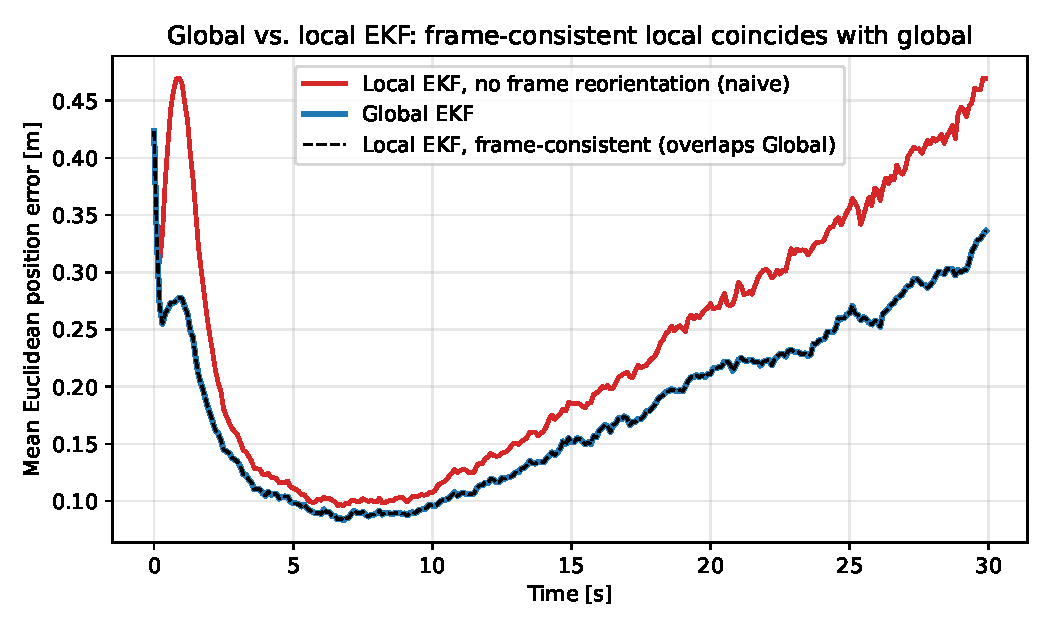
\includegraphics[width=0.82\linewidth]{Cap5/ekf_equivalence.pdf}
  \caption{Mean Euclidean position error over time. The global EKF and the
  frame-consistent local EKF coincide to machine precision (blue and dashed
  black). A local EKF that ignores the inter-frame reorientation
  (Section~\ref{sec:diverge}) is markedly worse (red).}
  \label{fig:ekf_equiv}
\end{figure}

\section{When the Formulations Diverge}
\label{sec:diverge}

Equivalence is a consequence of the three assumptions of
Proposition~\ref{prop:equiv}. Removing any of them yields a genuine difference,
and understanding these regimes is what actually guides the choice of frame.

\subsection{Neglecting Platform Motion}

If the reorientation \eqref{eq:reor_pos}--\eqref{eq:reor_cov} is omitted --- i.e.\
the moving body frame is implicitly treated as inertial --- the prediction is
biased by the platform displacement between consecutive steps. This single
omission raises the RMSE from $0.228$~m to $0.301$~m (the red curve in
Figure~\ref{fig:ekf_equiv}); it does \emph{not} reflect any intrinsic inferiority
of the local frame, but a modelling error. This regime is important precisely
because it can masquerade as a fair ``global versus local'' comparison and
produce a spurious advantage for the global formulation; the correct local filter
recovers the global filter's accuracy exactly.

\subsection{Anisotropic Process Noise}

Assumption~(ii) fails when the acceleration noise is directional in the inertial
frame --- for instance, a target that accelerates predominantly along its track.
Then $\bm{T}_k\bm{Q}\bm{T}_k^{\top}\neq\bm{Q}$, and the formulation whose frame
diagonalises $\bm{Q}$ is preferred: the global filter models inertial-frame
directional noise correctly, whereas the local filter injects it in the rotating
frame and is mismatched. With a strongly anisotropic intensity
($\sigma_{a,x}=0.6$, $\sigma_{a,y}=\sigma_{a,z}=0.05~\mathrm{m/s^2}$) and a
platform yawing at $0.6~\mathrm{rad/s}$, the global filter attains an RMSE of
$0.380$~m against $0.534$~m for the local filter --- a $41\%$ degradation
(Figure~\ref{fig:aniso}). Symmetrically, noise that is diagonal in the body frame
favours the local formulation. The guiding principle is to carry the state in the
frame where the process noise is naturally uncorrelated.

\begin{figure}[H]
  \centering
  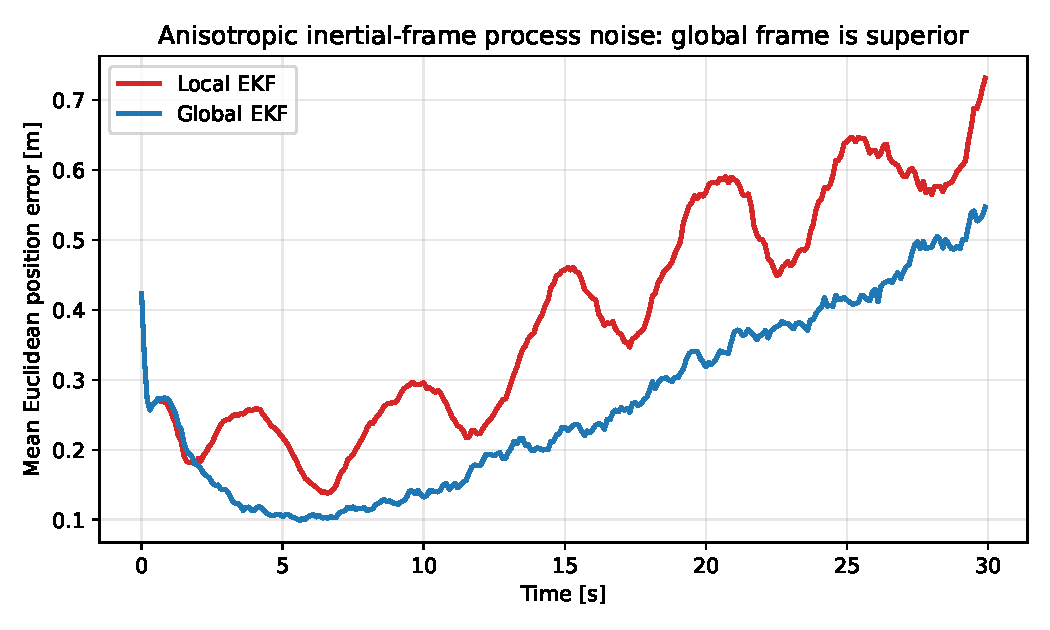
\includegraphics[width=0.82\linewidth]{Cap5/aniso_divergence.pdf}
  \caption{With anisotropic inertial-frame process noise and significant platform
  rotation, the equivalence breaks: the global EKF correctly models the
  directional acceleration noise and outperforms the local EKF.}
  \label{fig:aniso}
\end{figure}

\subsection{Uncertain Platform Pose}

Assumption~(i) is the most consequential in practice. When the platform pose is
\emph{estimated} rather than known, $(\bm{R}_k,\bm{p}^{p}_k)$ carry their own
uncertainty, which enters the global measurement equation \eqref{eq:hglobal} and
the local reorientation \eqref{eq:reor_pos} differently. The innovation covariance
\eqref{eq:gSK} must then be augmented with a term that propagates the pose
covariance, and the two formulations are no longer equivalent. This is the
setting of Chapter~\ref{cha:monocular}, where the monocular tracker explicitly propagates the
six-degree-of-freedom camera-pose uncertainty into the filter.

\section{Cram\'er--Rao Lower Bound}
\label{sec:crlb}

To benchmark the filters against the best achievable accuracy, we compute the
posterior Cram\'er--Rao bound (PCRB) for the discrete-time nonlinear
filtering problem \cite{tichavsky1998}. The Fisher information matrix obeys the
recursion
\begin{equation}
  \bm{J}_{k+1} = \big(\bm{F}\,\bm{J}_k^{-1}\,\bm{F}^{\top} + \bm{Q}\big)^{-1}
              + \mathbb{E}\!\big[\bm{H}_{k+1}^{\top}\,\bm{R}_{k+1}^{-1}\,\bm{H}_{k+1}\big],
  \label{eq:fim}
\end{equation}
where the expectation is taken over the state trajectory --- approximated by
Monte~Carlo, with $\bm{H}_{k+1}$ and $\bm{R}_{k+1}$ evaluated along each true
trajectory --- and the position bound is read off the inverse,
\begin{equation}
  \mathrm{PCRB}(k) = \big[\bm{J}_k^{-1}\big]_{1:3,\,1:3}.
  \label{eq:crlb}
\end{equation}
By Proposition~\ref{prop:equiv} the two formulations share the same bound.
Figure~\ref{fig:crlb} compares, per axis, the empirical RMSE of the filter (over
$3{,}000$ Monte~Carlo runs) with $\sqrt{\mathrm{PCRB}}$. The achieved error
remains at or above the bound at every step --- the filter is near-optimal ---
and the two grow together over time: as the object recedes from the
platform, the range $\rho$ increases and the heteroscedastic term
$\sigma_{\rho}^{2}=\alpha_{\rho}\rho^{2}$ in \eqref{eq:rangenoise} inflates the
measurement uncertainty. This growth is benign for sense-and-avoid: a distant
object poses a lower collision threat, so larger uncertainty at range is
acceptable.

\begin{figure}[H]
  \centering
  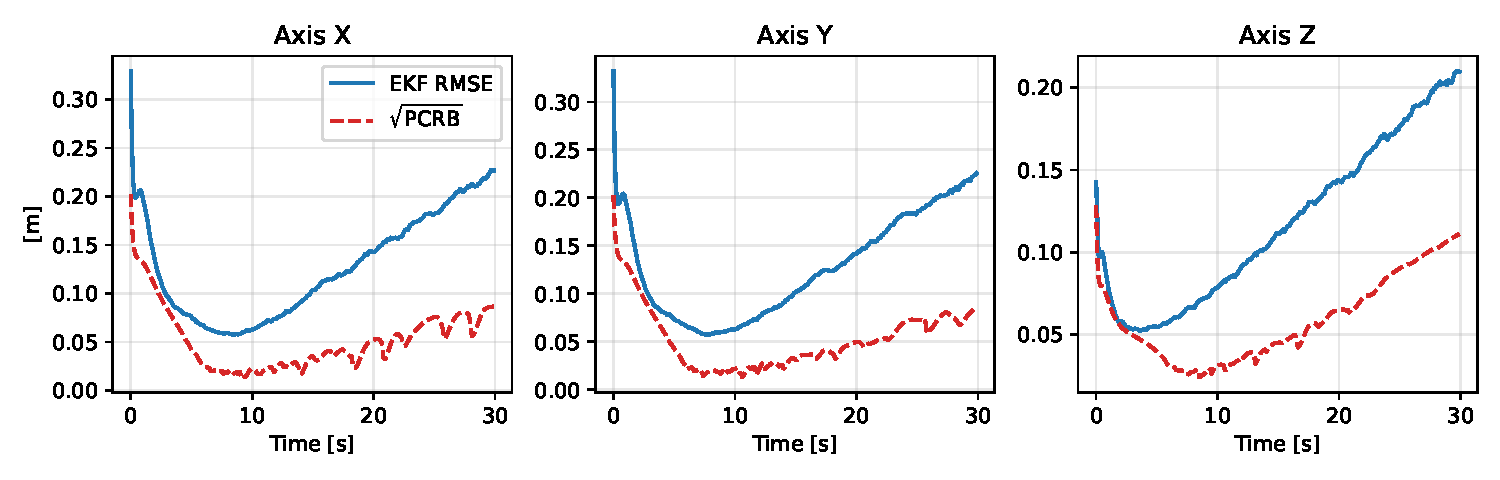
\includegraphics[width=\linewidth]{Cap5/crlb_vs_error.pdf}
  \caption{Per-axis RMSE of the EKF (blue) against the square root of the
  posterior Cram\'er--Rao bound (dashed red), over $3{,}000$ Monte~Carlo runs.
  The achieved error stays at or above the bound at every step; both grow with
  range because of the distance-dependent measurement noise \eqref{eq:rangenoise}.}
  \label{fig:crlb}
\end{figure}


\chapter{Extending the Tracker to Monocular Real-World Operation}\label{cha:monocular}
% =====================================================================
% Chapter 6 --- Monocular Person Tracking from a Moving UAV (TU Berlin)
%                                                            [tracker -- HERE]
% Self-contained project: Overview -> Methodology -> Results -> Discussion.
% Framed as an EXTENSION of Chapter~\ref{cha:tracking}: the same EKF framework
% generalises to a harder, monocular, real-world case and, because the platform
% pose is now uncertain, the global/local frames genuinely diverge here.
% Target length: ~9 pages (methodology + results).
% =====================================================================

\section{Overview and Objectives}
% TODO: the TU Berlin collaboration; from obstacle tracking to person tracking;
% generality of the framework of Chapter~\ref{cha:tracking}; camera-only sensing,
% ground-plane + known-height assumptions (no LiDAR).

\section{Methodology}

\subsection{Monocular Measurement Model and Plumb-Bob Undistortion}
% TODO: nonlinear pinhole projection as the measurement; iterative undistortion.

\subsection{Ground-Plane Constraint and Ray--Plane Initialization}
% TODO: target on plane z = z_obj; ray-plane lift of the first detection.

\subsection{Extrinsic-Aware Innovation Covariance}
% TODO: the core contribution -- propagate 6-DoF camera-pose uncertainty into the
% innovation covariance, S = H P H^T + J_ext Sigma_pose J_ext^T + R_cam.

\subsection{Temporal Synchronization}
% TODO: camera-to-pose latency compensation; SLERP/linear interpolation.

\subsection{Experimental Platform}
% TODO: custom quadrotor; global-shutter camera (IMX296); PX4/ASPN-PVT navigation feed.

\section{Results}

\subsection{Experimental Scenarios and Protocol}
% TODO: real flights; scenarios; ground-truth/annotation.

\subsection{Reprojection Error and Track Continuity}
% TODO

\subsection{Consistency under Platform Motion (NIS)}
% TODO: NIS over time; behaviour during aggressive platform motion.

\subsection{Ablation: Pose-Uncertainty On versus Off}
% TODO: the main ablation (Sigma_pose ON vs OFF).

\section{Discussion}
% TODO: connect back to Chapter~\ref{cha:tracking} -- this is precisely the regime
% (uncertain platform pose) where the global and local frames stop being equivalent --
% and to the pipeline (Chapter~\ref{cha:pipeline}).


\chapter{Synthetic Dataset and 3D Detection Pipeline}\label{cha:airsim}
% =====================================================================
% Chapter 7 --- Synthetic Dataset and 3D Detection Pipeline (AirSim)
%                                                       [detection -- OTHER PC]
% Self-contained project: Overview -> Dataset -> Detection methodology ->
% Results -> Discussion. This is the chapter completed on the other computer.
% Target length: ~9 pages (methodology + results).
% =====================================================================

\section{Overview and Objectives}
% TODO: motivation -- scarcity of annotated aerial 3D datasets; use AirSim to generate
% data and train the detection front-end of the pipeline (Chapter~\ref{cha:pipeline}).

\section{The AirSim Synthetic Dataset}

\subsection{Simulation Environment and Scenarios}
% TODO: AirSim/Unreal; urban scenarios; rationale for synthetic data and generalization.

\subsection{Sensor Channels and Annotations}
% TODO: RGB + depth + LiDAR + ego-pose; 2D/3D boxes, class, tracking IDs.

\subsection{Dataset Splits and Format}
% TODO: train/val/test; KITTI/nuScenes-compatible format.

\section{Detection Methodology}

\subsection{2D Detection}
% TODO: YOLO detector; inputs/outputs; training.

\subsection{Frustum Proposal}
% TODO: lifting 2D boxes into 3D frustums with camera intrinsics + point cloud.

\subsection{3D Detection with PointNet}
% TODO: PointNet on the frustum points; amodal 3D bounding box.

\section{Results}

\subsection{2D Detection Performance}
% TODO

\subsection{3D Detection Performance}
% TODO

\subsection{Generalization across Scenarios}
% TODO

\section{Discussion}
% TODO: how the trained detector feeds the tracker; sim-to-real outlook
% (link to the real-data tracking of Chapter~\ref{cha:monocular}).


\chapter{Conclusions and Future Work}\label{cha:conclusions}
% =====================================================================
% Chapter 8 --- Conclusions and Future Work                  [cross-cutting]
% Target length: ~4 pages.
% =====================================================================

\section{Summary of Contributions}
% TODO: revisit the contributions in light of the results.

\section{Limitations}
% TODO: honest limitations (e.g., real quantitative validation still maturing,
% detection-tracking integration not yet end-to-end on hardware).

\section{Future Work}
% TODO: real dataset from TU Berlin; full end-to-end pipeline integration;
% embedded deployment (Jetson); collaborative multi-UAV perception.


% REFERÊNCIAS BIBLIOGRÁFICAS
\renewcommand\bibname{\itareferencesnamebabel} % renomeia o título do capítulo de referências
\bibliography{Referencias/referencias}

% Apêndices
\appendix
\chapter{Detailed Jacobian and CRLB Derivations}
% =====================================================================
% Appendix A --- Detailed Jacobian and CRLB Derivations
% Goal: keep the body readable by moving long derivations here.
% =====================================================================

This appendix collects the derivations that the body chapters use but do not
spell out in full, so that the results of Chapters~\ref{cha:tracking}
and~\ref{cha:monocular} are reproducible. The notation is that of
Chapter~\ref{cha:background}.

\section{Spherical Measurement Jacobian}
\label{ap:spherical_jac}

The spherical measurement model maps a relative position in the sensor frame,
$\bm{p}^{c}=[x^{c},y^{c},z^{c}]^{\top}$, to range, azimuth and elevation,
\begin{equation}
  \rho = \sqrt{(x^{c})^{2}+(y^{c})^{2}+(z^{c})^{2}}, \quad
  \alpha = \operatorname{atan2}(y^{c},x^{c}), \quad
  \beta = \operatorname{atan2}\!\big(z^{c},\rho_{xy}\big),
\end{equation}
with $\rho_{xy}=\sqrt{(x^{c})^{2}+(y^{c})^{2}}$. Differentiating each component
with respect to the local Cartesian coordinates gives the rows of the
$3\times3$ Jacobian $\bm{J}_{\mathrm{s}}=\partial(\rho,\alpha,\beta)/\partial\bm{p}^{c}$.
For the range,
\begin{equation}
  \frac{\partial\rho}{\partial x^{c}}=\frac{x^{c}}{\rho},\qquad
  \frac{\partial\rho}{\partial y^{c}}=\frac{y^{c}}{\rho},\qquad
  \frac{\partial\rho}{\partial z^{c}}=\frac{z^{c}}{\rho}.
\end{equation}
For the azimuth, using $\tfrac{\partial}{\partial u}\operatorname{atan2}(v,u)=-v/(u^2+v^2)$ and
$\tfrac{\partial}{\partial v}\operatorname{atan2}(v,u)=u/(u^2+v^2)$,
\begin{equation}
  \frac{\partial\alpha}{\partial x^{c}}=\frac{-y^{c}}{\rho_{xy}^{2}},\qquad
  \frac{\partial\alpha}{\partial y^{c}}=\frac{x^{c}}{\rho_{xy}^{2}},\qquad
  \frac{\partial\alpha}{\partial z^{c}}=0.
\end{equation}
For the elevation $\beta=\operatorname{atan2}(z^{c},\rho_{xy})$, with
$\partial\rho_{xy}/\partial x^{c}=x^{c}/\rho_{xy}$ and similarly for $y^{c}$,
\begin{equation}
  \frac{\partial\beta}{\partial x^{c}}=\frac{-x^{c}z^{c}}{\rho^{2}\rho_{xy}},\qquad
  \frac{\partial\beta}{\partial y^{c}}=\frac{-y^{c}z^{c}}{\rho^{2}\rho_{xy}},\qquad
  \frac{\partial\beta}{\partial z^{c}}=\frac{\rho_{xy}}{\rho^{2}},
\end{equation}
so that, collecting the rows,
\begin{equation}
  \bm{J}_{\mathrm{s}} =
  \begin{bmatrix}
    \dfrac{x^{c}}{\rho} & \dfrac{y^{c}}{\rho} & \dfrac{z^{c}}{\rho}\\[8pt]
    \dfrac{-y^{c}}{\rho_{xy}^{2}} & \dfrac{x^{c}}{\rho_{xy}^{2}} & 0\\[8pt]
    \dfrac{-x^{c}z^{c}}{\rho^{2}\rho_{xy}} & \dfrac{-y^{c}z^{c}}{\rho^{2}\rho_{xy}} & \dfrac{\rho_{xy}}{\rho^{2}}
  \end{bmatrix},
\end{equation}
which is Eq.~\eqref{eq:Jsph}.

\paragraph*{Global- and local-frame measurement Jacobians.}
In the local formulation the state position is already expressed in the sensor
frame, so the $4\times7$ measurement Jacobian (with the size reading appended)
is $\bm{H}^{\mathrm{l}}_k=\big[\begin{smallmatrix}\bm{J}_{\mathrm{s}} & \bm{0}_{3\times3} & \bm{0}_{3\times1}\\ \bm{0}_{1\times3} & \bm{0}_{1\times3} & 1\end{smallmatrix}\big]$,
Eq.~\eqref{eq:Hlocal}. In the global formulation the predicted position is rotated
into the sensor frame first, $\bm{p}^{c}=\bm{R}_k^{\top}(\hat{\bm{p}}_{k|k-1}-\bm{p}^{p}_k)$,
so by the chain rule $\partial\bm{p}^{c}/\partial\bm{p}=\bm{R}_k^{\top}$ and
$\bm{H}^{\mathrm{g}}_k=\big[\begin{smallmatrix}\bm{J}_{\mathrm{s}}\bm{R}_k^{\top} & \bm{0}_{3\times3} & \bm{0}_{3\times1}\\ \bm{0}_{1\times3} & \bm{0}_{1\times3} & 1\end{smallmatrix}\big]$,
Eq.~\eqref{eq:Hglobal}. The two are related by $\bm{H}^{\mathrm{g}}_k=\bm{H}^{\mathrm{l}}_k\bm{T}_k$,
the identity used in the equivalence proof of Section~\ref{sec:equiv}.

\section{Rotation-Matrix Derivatives}
\label{ap:rot_jac}

For the $Z$--$Y$--$X$ convention $\bm{R}=\bm{R}_z(\psi)\bm{R}_y(\theta)\bm{R}_x(\phi)$
of Eq.~\eqref{eq:euler}, the derivative with respect to each Euler angle is
obtained by differentiating the corresponding elementary rotation and leaving the
others unchanged:
\begin{align}
  \frac{\partial\bm{R}}{\partial\phi} &= \bm{R}_z(\psi)\,\bm{R}_y(\theta)\,\bm{R}_x'(\phi), &
  \bm{R}_x'(\phi) &= \begin{bmatrix}0&0&0\\0&-s_\phi&-c_\phi\\0&c_\phi&-s_\phi\end{bmatrix},\\
  \frac{\partial\bm{R}}{\partial\theta} &= \bm{R}_z(\psi)\,\bm{R}_y'(\theta)\,\bm{R}_x(\phi), &
  \bm{R}_y'(\theta) &= \begin{bmatrix}-s_\theta&0&c_\theta\\0&0&0\\-c_\theta&0&-s_\theta\end{bmatrix},\\
  \frac{\partial\bm{R}}{\partial\psi} &= \bm{R}_z'(\psi)\,\bm{R}_y(\theta)\,\bm{R}_x(\phi), &
  \bm{R}_z'(\psi) &= \begin{bmatrix}-s_\psi&-c_\psi&0\\c_\psi&-s_\psi&0\\0&0&0\end{bmatrix},
\end{align}
with $c_\bullet=\cos$ and $s_\bullet=\sin$. These are needed whenever the platform
attitude is itself a state or an uncertain quantity; for the uncertain-pose
analysis of Chapter~\ref{cha:monocular} the more compact $SE(3)$ tangent-space
form of Section~\ref{ap:extrinsic_jac} is used instead.

\section{Recursive Posterior Cram\'er--Rao Bound}
\label{ap:crlb}

The posterior Cram\'er--Rao bound (PCRB) lower-bounds the error covariance of any
estimator of $\bm{x}_k$ from the measurements $\bm{z}_{1:k}$:
$\mathbb{E}\!\big[(\bm{x}_k-\hat{\bm{x}}_k)(\bm{x}_k-\hat{\bm{x}}_k)^{\top}\big]\succeq\bm{J}_k^{-1}$,
where $\bm{J}_k$ is the Bayesian (posterior) Fisher information matrix. For the
discrete-time system \eqref{eq:ss_process}--\eqref{eq:ss_meas} with additive
Gaussian process noise $\bm{Q}$ and measurement noise $\bm{R}_k$, Tichavsk\'y
\textit{et al.}\ \cite{tichavsky1998} show that $\bm{J}_k$ obeys the recursion
\begin{equation}
  \bm{J}_{k+1} = \big(\bm{Q}+\bm{F}\,\bm{J}_k^{-1}\,\bm{F}^{\top}\big)^{-1}
              + \mathbb{E}\!\big[\bm{H}_{k+1}^{\top}\bm{R}_{k+1}^{-1}\bm{H}_{k+1}\big],
  \label{ap:fim_rec}
\end{equation}
which is Eq.~\eqref{eq:fim}. The first term is the \emph{prediction} of the
information through the dynamics: it is the inverse of the predicted covariance
$\bm{Q}+\bm{F}\bm{J}_k^{-1}\bm{F}^{\top}$, exactly mirroring the Kalman time
update, and it can only \emph{reduce} the information, since the process noise
$\bm{Q}$ adds uncertainty. The second term is the \emph{information gain} from the
new measurement, the expected value of $\bm{H}^{\top}\bm{R}^{-1}\bm{H}$ over the
state trajectory; the expectation is what distinguishes the \emph{posterior} bound
from a single linearization, and is evaluated by Monte~Carlo over true
trajectories (Section~\ref{sec:crlb}), with $\bm{H}_{k+1}$ the measurement Jacobian
of Section~\ref{ap:spherical_jac} evaluated along each trajectory and $\bm{R}_{k+1}$
the range-dependent noise \eqref{eq:Rmatrix}. The position bound reported in
Chapter~\ref{cha:tracking} is the leading $3\times3$ block of $\bm{J}_k^{-1}$.

\section{Extrinsic Jacobian}
\label{ap:extrinsic_jac}

The monocular tracker of Chapter~\ref{cha:monocular} needs the sensitivity of the
predicted pixel to a perturbation of the camera pose. Write the on-plane target
point in the optical frame as $\bm{p}^{\mathcal{O}}=\bm{R}^{wo}_k\bm{X}^{\mathcal{W}}+\bm{t}^{wo}_k$,
and the pixel as $\bm{u}=\pi(\bm{K}\bm{p}^{\mathcal{O}})$. The Jacobian of the
projection with respect to the optical-frame point is
\begin{equation}
  \bm{J}_{\pi}=\frac{\partial\pi(\bm{K}\,\cdot)}{\partial\bm{p}^{\mathcal{O}}}
  = \begin{bmatrix}
      f_x/Z^{\mathcal{O}} & 0 & -f_x X^{\mathcal{O}}/(Z^{\mathcal{O}})^{2}\\[2pt]
      0 & f_y/Z^{\mathcal{O}} & -f_y Y^{\mathcal{O}}/(Z^{\mathcal{O}})^{2}
    \end{bmatrix},
\end{equation}
obtained by differentiating $\pi([X,Y,Z]^{\top})=[X/Z,\,Y/Z]^{\top}$ and scaling by
the focal lengths. A small pose perturbation is represented in the tangent space of
$SE(3)$ by $\bm{\xi}=[\bm{\delta\theta}^{\top}\ \bm{\delta t}^{\top}]^{\top}$, and
to first order it displaces the optical-frame point by
$\delta\bm{p}^{\mathcal{O}}\approx-[\bm{p}^{\mathcal{O}}]_\times\bm{\delta\theta}+\bm{\delta t}$
(Eq.~\eqref{eq:se3_pert}): a rotation error $\bm{\delta\theta}$ moves the point
along $-[\bm{p}^{\mathcal{O}}]_\times\bm{\delta\theta}$, and a translation error
$\bm{\delta t}$ moves it rigidly. Composing the two by the chain rule gives the
$2\times6$ extrinsic Jacobian of the pixel with respect to the pose,
\begin{equation}
  \bm{J}_{\mathrm{ext}}=\bm{J}_{\pi}\big[\,-[\bm{p}^{\mathcal{O}}]_\times \;\; \bm{I}_3\,\big],
\end{equation}
which is Eq.~\eqref{eq:Jext}. Modeling the navigation pose error as zero-mean
Gaussian with covariance $\bm{\Sigma}$, the first-order propagation
$\bm{J}_{\mathrm{ext}}\bm{\Sigma}\bm{J}_{\mathrm{ext}}^{\top}$ is the additive term
that inflates the innovation covariance \eqref{eq:Smono}.


\chapter{Dataset Details and Additional Results}
% =====================================================================
% Appendix B --- Dataset Details and Additional Results
% =====================================================================

This appendix records the configuration, training, and filter parameters needed
to reproduce the experiments of Chapters~\ref{cha:monocular} and~\ref{cha:airsim}.

\section{AirSim Dataset Configuration}
\label{ap:airsim_cfg}

\paragraph*{Environments and sensors.} The synthetic data of
Chapter~\ref{cha:airsim} were generated in three Unreal/AirSim environments,
\textsc{AirSimNH} (low-rise residential), \textsc{City} (dense downtown), and
\textsc{Coastline} (vegetated coastal). The ego platform carries an RGB camera, a
planar-depth camera, and a $64$-beam LiDAR, rigidly co-located ($0.35$~m forward,
$0.5$~m below the body origin) and pitched $-15^\circ$ so that they share one
optical frame. The camera is an ideal pinhole at $1280\times720$ with a
$90^\circ$ horizontal field of view ($f_x=f_y=640$~px, principal point
$(640,360)$~px, no lens distortion). Depth returns are kept for
$0.1\le z<250$~m, yielding $10^{5}$--$3\times10^{5}$ points per frame; the depth
camera, not the LiDAR, is the primary cloud, because at altitude the targets are
seen against the sky where the LiDAR returns nothing.

\paragraph*{Targets and 3D annotation.} Each target carries a visual quadrotor
mesh (\emph{VisQuad}) enlarged $\times4$ so as to be visible and densely sampled
at $20$--$100$~m; its axis-aligned full extents are $3.01\times3.93\times2.79$~m,
which after a $1.38$ margin (for the omitted spinning rotors) and halving give the
annotation half-extents $\bm{e}=[2.08,2.71,1.93]^{\top}$~m. The ground-truth 3D box
is built geometrically from the true global pose (not from the simulator's
detection API, which carries a systematic vertical offset). Per-frame acquisition
is performed with the scene frozen (\texttt{simPause}) and targets/ego
re-teleported to their planned poses, to keep image and reported poses consistent.

\paragraph*{Training and evaluation subsets.} The 2D detector is trained on
$\approx2{,}500$ pixel-exact synthetic-composition frames ($196$ drone sprites
spanning $12$~yaw~$\times$~$3$~pitch~$\times$~$3$~roll orientations at five ranges,
$1$--$5$ drones per frame). The point-cloud networks are trained on the collected
multimodal set ($3$ scenes $\times\,1{,}000$ frames). Evaluation uses a disjoint
campaign of $60$ video sequences ($20$ per environment, $75$--$110$ frames at
${\approx}5$~Hz) that randomizes the range regime (near $18$--$32$~m, mid
$32$--$50$~m, far $50$--$78$~m), time of day ($07$h--$18$h), weather (clear, light
fog, light rain), and number of targets ($2$--$3$), with a \emph{moving} observer.

\section{Network Training Hyperparameters}
\label{ap:train_hyper}

Table~\ref{tab:hyper_yolo} lists the 2D-detector training settings and
Table~\ref{tab:hyper_3d} the point-cloud--network settings, for reproducibility.

\begin{table}[H]
  \centering
  \footnotesize
  \caption{YOLOv11-small training (Ultralytics defaults unless noted): SGD with
  Nesterov momentum, weight decay, and a cosine learning-rate schedule.}
  \label{tab:hyper_yolo}
  \resizebox{\linewidth}{!}{%
  \begin{tabular}{@{}llll@{}}
    \toprule
    Setting & Synthetic drone (Ch.~\ref{cha:airsim}) & Real-urban drone (ref.) & Person (Ch.~\ref{cha:monocular}) \\
    \midrule
    Backbone        & YOLOv11s ($\approx 10$~M) & YOLOv11s & YOLOv11s \\
    Input size      & $1280$~px & $640$~px & $1280$~px \\
    Epochs          & $80$ & $100$ & $50$ \\
    Batch           & $16$ & $16$ & auto \\
    Patience        & default & $30$ & $100$ \\
    Pretrained      & COCO & COCO & COCO \\
    Augmentation    & mosaic, HSV, scale & mosaic, HSV, scale & Ultralytics default \\
    Result ($\mathrm{mAP}_{50}$) & $0.994$ & $0.731$ & $0.754$ \\
    \bottomrule
  \end{tabular}}
\end{table}

The Chapter~\ref{cha:monocular} person detector (rightmost column) was trained
through the Ultralytics HUB on the dataset \texttt{visdrone\_sard\_heridal}, the
union of the VisDrone, SARD, and HERIDAL aerial person-detection sets:
$14{,}783$ images of a single \texttt{person} class, split $74.1\%/12.4\%/13.5\%$
into train/validation/test ($10{,}961$, $1{,}829$, and $1{,}993$ images). Beyond
the $\mathrm{mAP}_{50}=0.754$ in the table, it reaches
$\mathrm{mAP}_{50\text{--}95}=0.389$, with precision $0.795$ and recall $0.669$ on
its validation split.

\begin{table}[H]
  \centering
  \footnotesize
  \caption{Point-cloud detector training. All use Adam ($10^{-3}$, weight decay
  $10^{-4}$) with a cosine schedule; frustum nets sample $N{=}4096$ points from
  the $25\%$-enlarged frustum and normalize by centroid subtraction and a scale.}
  \label{tab:hyper_3d}
  \begin{tabular}{@{}p{2.5cm} p{6.3cm} p{5.3cm}@{}}
    \toprule
    Network & Architecture (key) & Loss / schedule \\
    \midrule
    Frustum PointNet\texttt{++}
      & SA $[64,64,128]$ / $[128,128,256]$ / $[256,512,1024]$, FC $[512,256,128]$
      & Focal ($\alpha{=}0.5,\gamma{=}2$) $+\,5\,\mathrm{SL}_1(\text{ctr})+\mathrm{SL}_1(\text{size})$; $30$ ep., batch $8$ \\[2pt]
    T-Net segmentation
      & $+$ per-point fg/bg head ($1088{\to}256{\to}128{\to}1$)
      & $+\,\mathrm{BCE}(\text{seg})$; $20$ ep., batch $32$ \\[2pt]
    Frustum ConvNet
      & $16$ depth slices, per-slice mini-PointNet, $1$D conv
      & same heads; $30$ ep., batch $8$ \\[2pt]
    PointPillars (PFN)
      & BEV $1.25$~m grid, per-pillar mini-PointNet $[64,64]$, 2D CNN
      & center heatmap (focal) $+$ box reg.; $15$ ep., batch $8$ \\[2pt]
    Dense 3D voxel
      & $2.0$~m grid, Conv3D $1{\to}16{\to}32{\to}32{\to}64$
      & center heatmap $+$ box reg.; $15$ ep., batch $4$ \\
    \bottomrule
  \end{tabular}
\end{table}

\section{Filter Parameter Settings}
\label{ap:filter_params}

\paragraph*{3D range--bearing EKF (Chapters~\ref{cha:tracking} and~\ref{cha:airsim}).}
Acceleration intensity $\sigma_a=0.5~\mathrm{m/s^2}$; bearing noise
$\sigma_\alpha=\sigma_\beta=5~\mathrm{mrad}$; range noise $\sigma_\rho=0.05\,\rho$
(floored at $0.5$~m); size noise $\sigma_r=0.5$~m; initial position/velocity
standard deviations $5$~m / $10~\mathrm{m/s}$; gating at the $\chi^2$ $99\%$ level
($13.28$ for four degrees of freedom). The SORT-style association uses
non-maximum-suppression IoU $0.4$, association-gate IoU $0.3$, minimum hits $3$,
coasting horizon $4$, and maximum age $8$ frames (reproduced from
Table~\ref{tab:tracker}).

\paragraph*{Monocular ground-plane EKF (Chapter~\ref{cha:monocular}).}
Planar constant-velocity model with acceleration intensity $\sigma_a$; pixel
measurement noise $\bm{R}_{\mathrm{cam}}=\sigma_{\mathrm{cam}}^2\bm{I}_2$; the
$6$-DoF pose covariance is modeled as isotropic,
$\bm{\Sigma}=\sigma_{\mathrm{pose}}^2\bm{I}_6$, with $\sigma_{\mathrm{pose}}$ tuned
by the NIS consistency analysis of Section~\ref{sec:mono_consistency} to
$\sigma_{\mathrm{pose}}\approx10^{-3}$, the value at which the mean NIS crosses the
consistent value $\bar\eta=2$. The first detection is initialized by ray--plane
intersection with a large initial covariance so that early measurements dominate.

\section{Code and Data Availability}
\label{ap:code}

The synthetic-dataset generation and 3D-detection pipeline of
Chapter~\ref{cha:airsim} are released as open source at
\url{https://github.com/ericyoshida/airsim-uav-3d-detection}. The monocular
tracker of Chapter~\ref{cha:monocular} is available from the author on request;
its public release, together with any TU~Berlin flight data, is subject to the
consent of the collaborating team. In both cases the large artifacts (datasets,
model weights, recordings) are kept separate from the code.


% Anexos (opcional)
% \annex
% \chapter{...}
% \input{AneA/anexoA}

% Glossário (opcional)
%\itaglossary
%\printglossary

% Folha de Registro do Documento (FRD)
\FRDitadata{28 de julho de 2026}
\FRDitadocnro{DCTA/ITA/DM - XXX/2026}                            % TODO: número de registro solicitado à biblioteca
\FRDitaorgaointerno{Instituto Tecnológico de Aeronáutica -- ITA}
\FRDitapalavrasautor{Unmanned aerial vehicles; Detect-and-avoid; Object tracking; Extended Kalman filter; 3D object detection; Sensor fusion; Convolutional neural networks.}
\FRDitapalavrasresult{Aeronaves não-tripuladas; Rastreamento; Filtro de Kalman estendido; Redes neurais convolucionais; Visão computacional; Fusão de sensores; Métodos computacionais.}
\FRDitapalavraapresentacao{ITA, São José dos Campos. Curso de Mestrado. Programa de Pós-Graduação em Electronic Engineering and Computer Science. Área de Informatics. Orientador: Prof.~Dr.~Marcos Ricardo Omena de Albuquerque Maximo; Coorientador: Dr.~Stiven Schwanz Dias. Defesa em 28/07/2026.}
\FRDitaresumo{% Resumo condensado para a Folha de Registro do Documento (FRD).
% A caixa "RESUMO" da FRD tem altura fixa; o resumo completo (PreTextuais/resumo.tex)
% não cabe nela, por isso esta versão reduzida.

Esta dissertação desenvolve a camada de percepção (\emph{sense}) do
\emph{detect-and-avoid} de veículos aéreos não tripulados urbanos, estruturada
como um pipeline modular câmera--nuvem de pontos: uma rede neural convolucional
localiza o obstáculo na imagem, a região detectada é estendida para o espaço como
um tronco de visada (\emph{frustum}) que recorta a nuvem de pontos, uma segunda
rede ajusta uma caixa tridimensional métrica, e um Filtro de Kalman Estendido
converte as detecções em trajetórias com incerteza calibrada. Três estudos
autocontidos validam o pipeline. O primeiro formula o rastreamento a partir de
uma plataforma em movimento nos referenciais global e local, prova que as duas
formulações são matematicamente equivalentes sob pose conhecida e ruído de
processo isotrópico, caracteriza os regimes em que essa equivalência falha, e
mostra que o filtro é quase ótimo frente ao limite de Cramér--Rao posterior. O
segundo leva o mesmo estimador a voos reais de um quadrimotor, rastreando uma
pessoa com uma única câmera e pose estimada a bordo, e demonstra que propagar a
incerteza de pose para a inovação é necessário para a consistência estatística.
O terceiro constrói um conjunto de dados sintético no simulador AirSim, treina os
estágios de detecção e identifica a extração de \emph{foreground}, e não o
regressor da caixa, como o fator dominante na acurácia de localização 3D.
}
%  Primeiro parametro: Nacional ou Internacional -- N/I
%  Segundo parametro: Ostensivo, Reservado, Confidencial ou Secreto -- O/R/C/S
\FRDitaOpcoes{N}{O}
\itaFRD

\end{document}
